\documentclass[ignorenonframetext,]{beamer}
\setbeamertemplate{caption}[numbered]
\setbeamertemplate{caption label separator}{: }
\setbeamercolor{caption name}{fg=normal text.fg}
\beamertemplatenavigationsymbolsempty
\usepackage{lmodern}
\usepackage{amssymb,amsmath}
\usepackage{ifxetex,ifluatex}
\usepackage{fixltx2e} % provides \textsubscript
\ifnum 0\ifxetex 1\fi\ifluatex 1\fi=0 % if pdftex
  \usepackage[T1]{fontenc}
  \usepackage[utf8]{inputenc}
\else % if luatex or xelatex
  \ifxetex
    \usepackage{mathspec}
  \else
    \usepackage{fontspec}
  \fi
  \defaultfontfeatures{Ligatures=TeX,Scale=MatchLowercase}
\fi
% use upquote if available, for straight quotes in verbatim environments
\IfFileExists{upquote.sty}{\usepackage{upquote}}{}
% use microtype if available
\IfFileExists{microtype.sty}{%
\usepackage{microtype}
\UseMicrotypeSet[protrusion]{basicmath} % disable protrusion for tt fonts
}{}
\newif\ifbibliography
\hypersetup{
            pdftitle={Análisis discriminante},
            pdfauthor={Dr.~Luis Benites},
            pdfborder={0 0 0},
            breaklinks=true}
\urlstyle{same}  % don't use monospace font for urls
\usepackage{color}
\usepackage{fancyvrb}
\newcommand{\VerbBar}{|}
\newcommand{\VERB}{\Verb[commandchars=\\\{\}]}
\DefineVerbatimEnvironment{Highlighting}{Verbatim}{commandchars=\\\{\}}
% Add ',fontsize=\small' for more characters per line
\usepackage{framed}
\definecolor{shadecolor}{RGB}{248,248,248}
\newenvironment{Shaded}{\begin{snugshade}}{\end{snugshade}}
\newcommand{\KeywordTok}[1]{\textcolor[rgb]{0.13,0.29,0.53}{\textbf{#1}}}
\newcommand{\DataTypeTok}[1]{\textcolor[rgb]{0.13,0.29,0.53}{#1}}
\newcommand{\DecValTok}[1]{\textcolor[rgb]{0.00,0.00,0.81}{#1}}
\newcommand{\BaseNTok}[1]{\textcolor[rgb]{0.00,0.00,0.81}{#1}}
\newcommand{\FloatTok}[1]{\textcolor[rgb]{0.00,0.00,0.81}{#1}}
\newcommand{\ConstantTok}[1]{\textcolor[rgb]{0.00,0.00,0.00}{#1}}
\newcommand{\CharTok}[1]{\textcolor[rgb]{0.31,0.60,0.02}{#1}}
\newcommand{\SpecialCharTok}[1]{\textcolor[rgb]{0.00,0.00,0.00}{#1}}
\newcommand{\StringTok}[1]{\textcolor[rgb]{0.31,0.60,0.02}{#1}}
\newcommand{\VerbatimStringTok}[1]{\textcolor[rgb]{0.31,0.60,0.02}{#1}}
\newcommand{\SpecialStringTok}[1]{\textcolor[rgb]{0.31,0.60,0.02}{#1}}
\newcommand{\ImportTok}[1]{#1}
\newcommand{\CommentTok}[1]{\textcolor[rgb]{0.56,0.35,0.01}{\textit{#1}}}
\newcommand{\DocumentationTok}[1]{\textcolor[rgb]{0.56,0.35,0.01}{\textbf{\textit{#1}}}}
\newcommand{\AnnotationTok}[1]{\textcolor[rgb]{0.56,0.35,0.01}{\textbf{\textit{#1}}}}
\newcommand{\CommentVarTok}[1]{\textcolor[rgb]{0.56,0.35,0.01}{\textbf{\textit{#1}}}}
\newcommand{\OtherTok}[1]{\textcolor[rgb]{0.56,0.35,0.01}{#1}}
\newcommand{\FunctionTok}[1]{\textcolor[rgb]{0.00,0.00,0.00}{#1}}
\newcommand{\VariableTok}[1]{\textcolor[rgb]{0.00,0.00,0.00}{#1}}
\newcommand{\ControlFlowTok}[1]{\textcolor[rgb]{0.13,0.29,0.53}{\textbf{#1}}}
\newcommand{\OperatorTok}[1]{\textcolor[rgb]{0.81,0.36,0.00}{\textbf{#1}}}
\newcommand{\BuiltInTok}[1]{#1}
\newcommand{\ExtensionTok}[1]{#1}
\newcommand{\PreprocessorTok}[1]{\textcolor[rgb]{0.56,0.35,0.01}{\textit{#1}}}
\newcommand{\AttributeTok}[1]{\textcolor[rgb]{0.77,0.63,0.00}{#1}}
\newcommand{\RegionMarkerTok}[1]{#1}
\newcommand{\InformationTok}[1]{\textcolor[rgb]{0.56,0.35,0.01}{\textbf{\textit{#1}}}}
\newcommand{\WarningTok}[1]{\textcolor[rgb]{0.56,0.35,0.01}{\textbf{\textit{#1}}}}
\newcommand{\AlertTok}[1]{\textcolor[rgb]{0.94,0.16,0.16}{#1}}
\newcommand{\ErrorTok}[1]{\textcolor[rgb]{0.64,0.00,0.00}{\textbf{#1}}}
\newcommand{\NormalTok}[1]{#1}
\usepackage{graphicx,grffile}
\makeatletter
\def\maxwidth{\ifdim\Gin@nat@width>\linewidth\linewidth\else\Gin@nat@width\fi}
\def\maxheight{\ifdim\Gin@nat@height>\textheight0.8\textheight\else\Gin@nat@height\fi}
\makeatother
% Scale images if necessary, so that they will not overflow the page
% margins by default, and it is still possible to overwrite the defaults
% using explicit options in \includegraphics[width, height, ...]{}
\setkeys{Gin}{width=\maxwidth,height=\maxheight,keepaspectratio}

% Prevent slide breaks in the middle of a paragraph:
\widowpenalties 1 10000
\raggedbottom

\AtBeginPart{
  \let\insertpartnumber\relax
  \let\partname\relax
  \frame{\partpage}
}
\AtBeginSection{
  \ifbibliography
  \else
    \let\insertsectionnumber\relax
    \let\sectionname\relax
    \frame{\sectionpage}
  \fi
}
\AtBeginSubsection{
  \let\insertsubsectionnumber\relax
  \let\subsectionname\relax
  \frame{\subsectionpage}
}

\setlength{\parindent}{0pt}
\setlength{\parskip}{6pt plus 2pt minus 1pt}
\setlength{\emergencystretch}{3em}  % prevent overfull lines
\providecommand{\tightlist}{%
  \setlength{\itemsep}{0pt}\setlength{\parskip}{0pt}}
\setcounter{secnumdepth}{0}

\title{Análisis discriminante}
\author{Dr.~Luis Benites}
\date{26 de octubre del 2019}

\begin{document}
\frame{\titlepage}

\begin{frame}{Análisis Discriminante Lineal}

\begin{itemize}
\tightlist
\item
  Supongamos que un conjunto de objetos se clasifica en una serie de
  grupos; el Análisis Discriminante equivale a un análisis de regresión
  donde la variable dependiente es categórica y tiene como categorías la
  etiqueta de cada uno de los grupos, y las variables independientes son
  continuas y determinan a qué grupos pertenecen los objetos.
\end{itemize}

\end{frame}

\begin{frame}{Análisis Discriminante Lineal}

\begin{itemize}
\tightlist
\item
  Se trata de encontrar relaciones lineales entre las variables
  continuas que mejor discriminen en los grupos dados a los objetos.
  Además, se trata de definir una regla de decisión que asigne un objeto
  nuevo, que no sabemos clasificar previamente, a uno de los grupos
  prefijados.
\end{itemize}

\end{frame}

\begin{frame}{Análisis Discriminante Lineal}

\begin{itemize}
\item
  Se presentan una serie de restricciones o supuestos:

  \begin{itemize}
  \tightlist
  \item
    Se tiene una variable categórica y el resto de variables son de
    intervalo o de razón y son independientes respecto de ella.
  \item
    Es necesario que existan al menos dos grupos y para cada grupo se
    necesitan dos o más casos.
  \item
    El número de variables discriminantes debe ser menor que el número
    de objetos menos dos: \(x_1, \ldots , x_p\) donde \(p<(n-2)\) y
    \(n\) es el número de objetos.
  \end{itemize}
\end{itemize}

\end{frame}

\begin{frame}{Análisis Discriminante Lineal}

\begin{itemize}
\item
  Se presentan una serie de restricciones o supuestos:

  \begin{itemize}
  \tightlist
  \item
    Ninguna variable discriminante puede ser combinación lineal de otras
    variables discriminantes.
  \item
    El número máximo de funciones discriminantes es igual al mínimo
    entre el número de variables y el número de grupos menos 1 (con
    \(q\) grupos, (\(q-1\)) funciones discriminantes)
  \end{itemize}
\end{itemize}

\end{frame}

\begin{frame}{Análisis Discriminante Lineal}

\begin{itemize}
\item
  Las condiciones que se deben cumplir para que un Análisis
  Discriminante Lineal sea válido son:

  \begin{itemize}
  \tightlist
  \item
    Cada predictor que forma parte del modelo se distribuye de forma
    normal en cada una de las clases de la variable respuesta. En el
    caso de múltiples predictores, las observaciones siguen una
    distribución normal multivariante en todas las clases.
  \end{itemize}
\end{itemize}

\end{frame}

\begin{frame}{Análisis Discriminante Lineal}

\begin{itemize}
\item
  Las condiciones que se deben cumplir para que un Análisis
  Discriminante Lineal sea válido son:

  \begin{itemize}
  \tightlist
  \item
    La varianza del predictor es igual en todas las clases de la
    variable respuesta. En el caso de múltiples predictores, la matriz
    de covarianza es igual en todas las clases. Si esto no se cumple se
    recurre a Análisis Discriminante Cuadrático (QDA).
  \end{itemize}
\end{itemize}

\end{frame}

\begin{frame}{Análisis Discriminante Lineal}

\begin{itemize}
\item
  Las condiciones que se deben cumplir para que un Análisis
  Discriminante Lineal sea válido son:

  \begin{itemize}
  \tightlist
  \item
    Cuando la condición de normalidad no se cumple, el LDA pierde
    precisión pero aun así puede llegar a clasificaciones relativamente
    buenas. Using discriminant analysis for multi-class classification:
    an experimental investigation (Tao Li, Shenghuo Zhu, Mitsunori
    Ogihara).
  \end{itemize}
\end{itemize}

\end{frame}

\begin{frame}{Ejemplo 1}

\begin{itemize}
\item
  Se consideran los datos recogidos sobre 32 cráneos en el Tibet.
\item
  Los datos corresponden a dos tipos raciales diferentes en los que se
  practicaron diferentes medidas antropométricas de longitudes, anchuras
  de cráneo y de cara. Se trata de hacer un análisis discriminante sobre
  los dos tipos raciales.
\end{itemize}

\end{frame}

\begin{frame}[fragile]{cargando el conjunto de datos}

\begin{Shaded}
\begin{Highlighting}[]
\NormalTok{craneo <-}\StringTok{ }\KeywordTok{read.table}\NormalTok{(}\StringTok{"craneo.txt"}\NormalTok{,}\DataTypeTok{header=}\NormalTok{T)}
\NormalTok{craneo}
\end{Highlighting}
\end{Shaded}

\begin{verbatim}
##    Longitud Anchura Altura Altura_Cara Anchura_Cara Tipo
## 1     190.5   152.5  145.0        73.5        136.5  uno
## 2     172.5   132.0  125.5        63.0        121.0  uno
## 3     167.0   130.0  125.5        69.5        119.5  uno
## 4     169.5   150.5  133.5        64.5        128.0  uno
## 5     175.0   138.5  126.0        77.5        135.5  uno
## 6     177.5   142.5  142.5        71.5        131.0  uno
## 7     179.5   142.5  127.5        70.5        134.5  uno
## 8     179.5   138.0  133.5        73.5        132.5  uno
## 9     173.5   135.5  130.5        70.0        133.5  uno
## 10    162.5   139.0  131.0        62.0        126.0  uno
## 11    178.5   135.0  136.0        71.0        124.0  uno
## 12    171.5   148.5  132.5        65.0        146.5  uno
## 13    180.5   139.0  132.0        74.5        134.5  uno
## 14    183.0   149.0  121.5        76.5        142.0  uno
## 15    169.5   130.0  131.0        68.0        119.0  uno
## 16    172.0   140.0  136.0        70.5        133.5  uno
## 17    170.0   126.5  134.5        66.0        118.5  uno
## 18    182.5   136.0  138.5        76.0        134.0  dos
## 19    179.5   135.0  128.5        74.0        132.0  dos
## 20    191.0   140.5  140.5        72.5        131.5  dos
## 21    184.5   141.5  134.5        76.5        141.5  dos
## 22    181.0   142.0  132.5        79.0        136.5  dos
## 23    173.5   136.5  126.0        71.5        136.5  dos
## 24    188.5   130.0  143.0        79.5        136.0  dos
## 25    175.0   153.0  130.0        76.5        142.0  dos
## 26    196.0   142.5  123.5        76.0        134.0  dos
## 27    200.0   139.5  143.5        82.5        146.0  dos
## 28    185.0   134.5  140.0        81.5        137.0  dos
## 29    174.5   143.5  132.5        74.0        136.5  dos
## 30    195.5   144.0  138.5        78.5        144.0  dos
## 31    197.0   131.5  135.0        80.5        139.0  dos
## 32    182.5   131.0  135.0        68.5        136.0  dos
\end{verbatim}

\end{frame}

\begin{frame}[fragile]{Exploración gráfica de los datos}

\begin{Shaded}
\begin{Highlighting}[]
\KeywordTok{library}\NormalTok{(ggplot2)}
\KeywordTok{library}\NormalTok{(ggpubr)}
\NormalTok{p1 <-}\StringTok{ }\KeywordTok{ggplot}\NormalTok{(}\DataTypeTok{data =}\NormalTok{ craneo, }\KeywordTok{aes}\NormalTok{(}\DataTypeTok{x =}\NormalTok{ Longitud, }\DataTypeTok{fill =}\NormalTok{ Tipo)) }\OperatorTok{+}
\StringTok{  }\KeywordTok{geom_histogram}\NormalTok{(}\DataTypeTok{position =} \StringTok{"identity"}\NormalTok{, }\DataTypeTok{alpha =} \FloatTok{0.5}\NormalTok{)}
\NormalTok{p2 <-}\StringTok{ }\KeywordTok{ggplot}\NormalTok{(}\DataTypeTok{data =}\NormalTok{ craneo, }\KeywordTok{aes}\NormalTok{(}\DataTypeTok{x =}\NormalTok{ Anchura, }\DataTypeTok{fill =}\NormalTok{ Tipo)) }\OperatorTok{+}
\StringTok{  }\KeywordTok{geom_histogram}\NormalTok{(}\DataTypeTok{position =} \StringTok{"identity"}\NormalTok{, }\DataTypeTok{alpha =} \FloatTok{0.5}\NormalTok{)}
\NormalTok{p3 <-}\StringTok{ }\KeywordTok{ggplot}\NormalTok{(}\DataTypeTok{data =}\NormalTok{ craneo, }\KeywordTok{aes}\NormalTok{(}\DataTypeTok{x =}\NormalTok{ Altura, }\DataTypeTok{fill =}\NormalTok{ Tipo)) }\OperatorTok{+}
\StringTok{  }\KeywordTok{geom_histogram}\NormalTok{(}\DataTypeTok{position =} \StringTok{"identity"}\NormalTok{, }\DataTypeTok{alpha =} \FloatTok{0.5}\NormalTok{)}
\NormalTok{p4 <-}\StringTok{ }\KeywordTok{ggplot}\NormalTok{(}\DataTypeTok{data =}\NormalTok{ craneo, }\KeywordTok{aes}\NormalTok{(}\DataTypeTok{x =}\NormalTok{ Altura_Cara, }\DataTypeTok{fill =}\NormalTok{ Tipo)) }\OperatorTok{+}
\StringTok{  }\KeywordTok{geom_histogram}\NormalTok{(}\DataTypeTok{position =} \StringTok{"identity"}\NormalTok{, }\DataTypeTok{alpha =} \FloatTok{0.5}\NormalTok{)}
\NormalTok{p5 <-}\StringTok{ }\KeywordTok{ggplot}\NormalTok{(}\DataTypeTok{data =}\NormalTok{ craneo, }\KeywordTok{aes}\NormalTok{(}\DataTypeTok{x =}\NormalTok{ Anchura_Cara, }\DataTypeTok{fill =}\NormalTok{ Tipo)) }\OperatorTok{+}
\StringTok{  }\KeywordTok{geom_histogram}\NormalTok{(}\DataTypeTok{position =} \StringTok{"identity"}\NormalTok{, }\DataTypeTok{alpha =} \FloatTok{0.5}\NormalTok{)}
\KeywordTok{ggarrange}\NormalTok{(p1, p2, p3, p4, p5, }\DataTypeTok{nrow =} \DecValTok{5}\NormalTok{, }\DataTypeTok{common.legend =} \OtherTok{TRUE}\NormalTok{)}
\end{Highlighting}
\end{Shaded}

\end{frame}

\begin{frame}{Exploración gráfica de los datos}

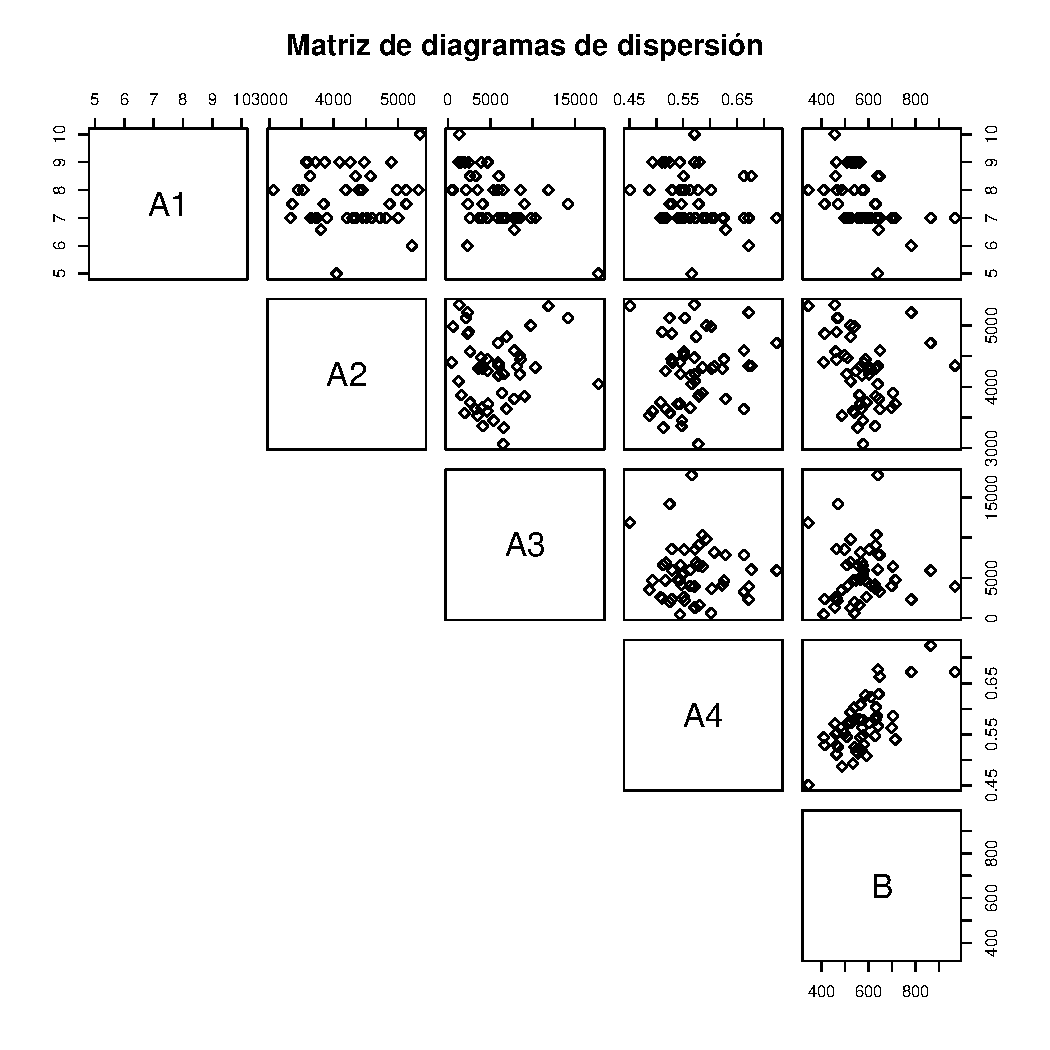
\includegraphics{LDA_files/figure-beamer/unnamed-chunk-2-1.pdf}

\end{frame}

\begin{frame}{Exploración gráfica de los datos}

\hypertarget{left}{}
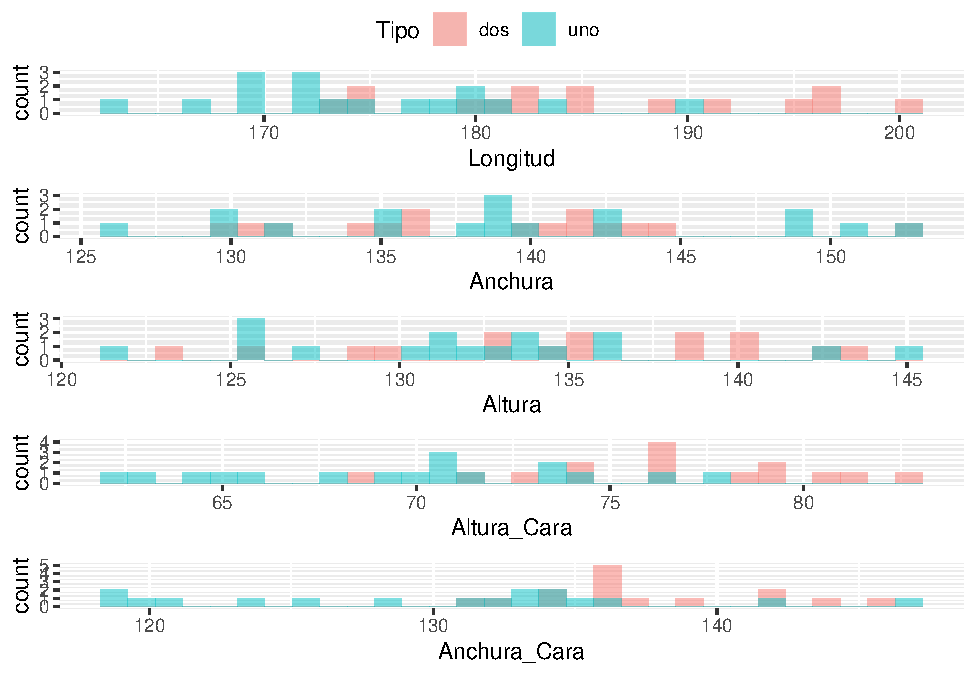
\includegraphics{LDA_files/figure-beamer/unnamed-chunk-3-1.pdf}

\hypertarget{right}{}
A nivel individual, la anchura de la cara parece ser la variable que más
se diferencia entre los dos tipos raciales.

(menor solapamiento entre poblaciones)

Seguida de las variables anchura de la cara y longitud del craneo que
también se diferencia entre los dos tipos raciales.

\end{frame}

\begin{frame}{Exploración gráfica de los datos}

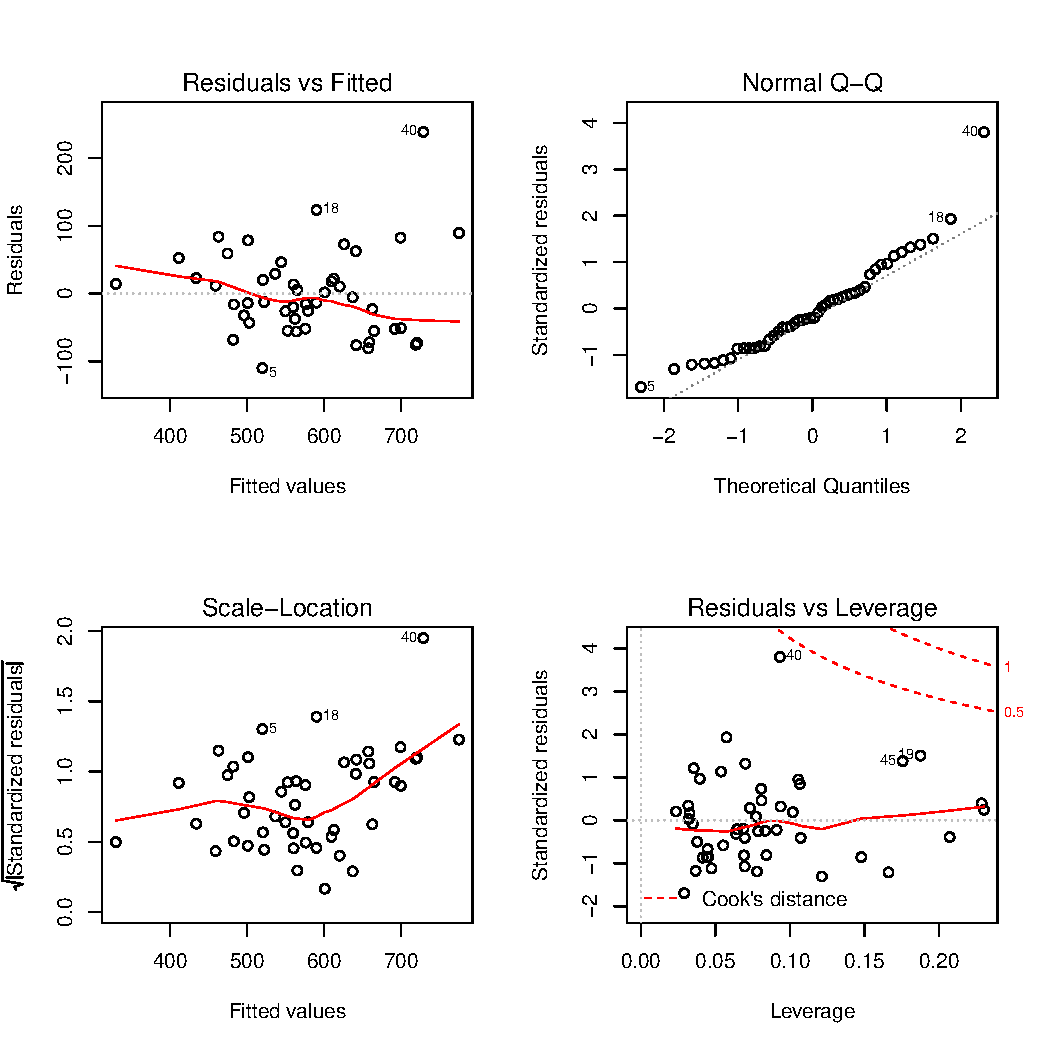
\includegraphics{LDA_files/figure-beamer/unnamed-chunk-4-1.pdf}

\end{frame}

\begin{frame}[fragile]{Exploración gráfica de los datos}

\hypertarget{left}{}
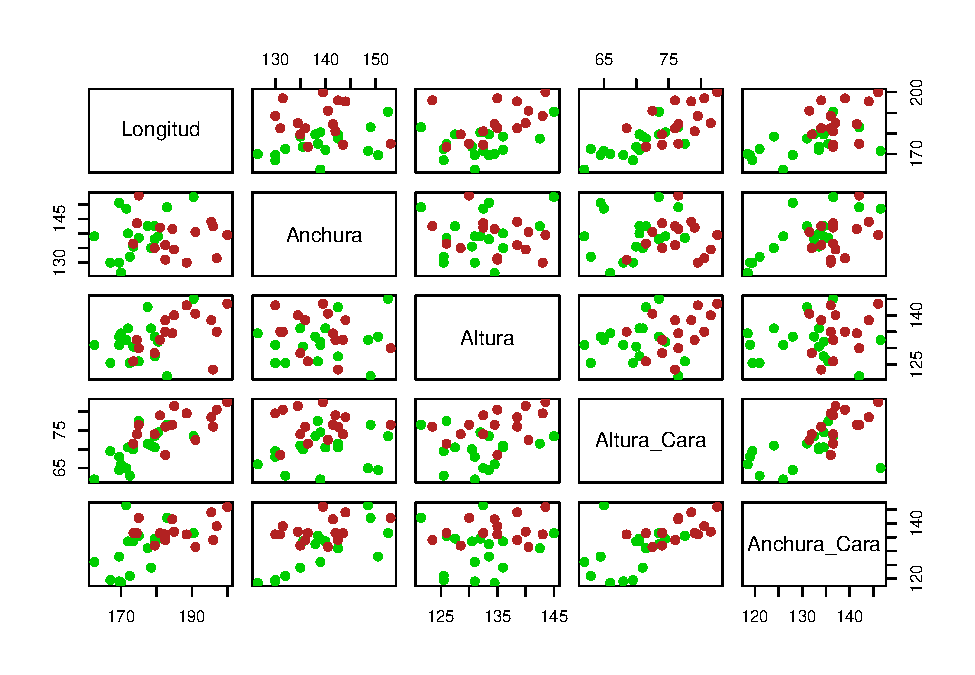
\includegraphics{LDA_files/figure-beamer/unnamed-chunk-5-1.pdf}

\hypertarget{right}{}
\begin{Shaded}
\begin{Highlighting}[]
\KeywordTok{pairs}\NormalTok{(}\DataTypeTok{x =}\NormalTok{ craneo[, }\KeywordTok{c}\NormalTok{(}\StringTok{"Longitud"}\NormalTok{, }\StringTok{"Anchura"}\NormalTok{, }\StringTok{"Altura"}\NormalTok{, }\StringTok{"Altura_Cara"}\NormalTok{, }\StringTok{"Anchura_Cara"}\NormalTok{)],}
      \DataTypeTok{col =} \KeywordTok{c}\NormalTok{(}\StringTok{"firebrick"}\NormalTok{, }\StringTok{"green3"}\NormalTok{)[craneo}\OperatorTok{$}\NormalTok{Tipo], }\DataTypeTok{pch =} \DecValTok{19}\NormalTok{)}
\end{Highlighting}
\end{Shaded}

Las variables altura de cara y anchura de cara tienen potencial para
poder separar los tipos de raza. Sin embargo, parecen estar altamente
correlacionadas, por lo que la información que aportan es redundante.

Las variables altura de cara y anchura de cara tienen potencial para
poder separar los tipos de raza. Sin embargo, parecen estar altamente
correlacionadas, por lo que la información que aportan es redundante.

Las variables altura y altura de cara también tienen potencial para
poder separar los tipos de raza.

La variable longitud cruzada con el resto de variables también muestra
potencial para separar los tipos de raza.

\end{frame}

\begin{frame}[fragile]{Probabilidades a priori}

Como no se dispone de información sobre la abundancia relativa de los
tipos raciales a nivel poblacional, se considera como probabilidad
previa de cada especie el número de observaciones del tipo racial entre
el número de observaciones totales.

\begin{Shaded}
\begin{Highlighting}[]
\KeywordTok{table}\NormalTok{(craneo}\OperatorTok{$}\NormalTok{Tipo)}\OperatorTok{/}\KeywordTok{nrow}\NormalTok{(craneo)}
\end{Highlighting}
\end{Shaded}

\begin{verbatim}
## 
##     dos     uno 
## 0.46875 0.53125
\end{verbatim}

\[\hat{\pi}_{uno}=0.53 \quad \text{y} \quad \hat{\pi}_{dos}=0.47\]

\end{frame}

\begin{frame}[fragile]{Normalidad univariante}

\begin{Shaded}
\begin{Highlighting}[]
\CommentTok{# Representación mediante Histograma de cada variable para cada tipo }
\KeywordTok{par}\NormalTok{(}\DataTypeTok{mfcol =} \KeywordTok{c}\NormalTok{(}\DecValTok{2}\NormalTok{, }\DecValTok{5}\NormalTok{))}
\ControlFlowTok{for}\NormalTok{ (k }\ControlFlowTok{in} \DecValTok{1}\OperatorTok{:}\DecValTok{5}\NormalTok{) \{}
\NormalTok{  j0 <-}\StringTok{ }\KeywordTok{names}\NormalTok{(craneo)[k]}
\NormalTok{  x0 <-}\StringTok{ }\KeywordTok{seq}\NormalTok{(}\KeywordTok{min}\NormalTok{(craneo[, k]), }\KeywordTok{max}\NormalTok{(craneo[, k]), }\DataTypeTok{le =} \DecValTok{1000}\NormalTok{)}
  \ControlFlowTok{for}\NormalTok{ (i }\ControlFlowTok{in} \DecValTok{1}\OperatorTok{:}\DecValTok{2}\NormalTok{) \{}
\NormalTok{    i0 <-}\StringTok{ }\KeywordTok{levels}\NormalTok{(craneo}\OperatorTok{$}\NormalTok{Tipo)[i]}
\NormalTok{    x <-}\StringTok{ }\NormalTok{craneo[craneo}\OperatorTok{$}\NormalTok{Tipo }\OperatorTok{==}\StringTok{ }\NormalTok{i0, j0]}
    \KeywordTok{hist}\NormalTok{(x, }\DataTypeTok{proba =}\NormalTok{ T, }\DataTypeTok{col =} \KeywordTok{grey}\NormalTok{(}\FloatTok{0.8}\NormalTok{), }\DataTypeTok{main =} \KeywordTok{paste}\NormalTok{(}\StringTok{"Tipo"}\NormalTok{, i0),}
         \DataTypeTok{xlab =}\NormalTok{ j0)}
    \KeywordTok{lines}\NormalTok{(x0, }\KeywordTok{dnorm}\NormalTok{(x0, }\KeywordTok{mean}\NormalTok{(x), }\KeywordTok{sd}\NormalTok{(x)), }\DataTypeTok{col =} \StringTok{"red"}\NormalTok{, }\DataTypeTok{lwd =} \DecValTok{2}\NormalTok{)}
\NormalTok{  \}}
\NormalTok{\}}
\KeywordTok{par}\NormalTok{(}\DataTypeTok{mfcol =} \KeywordTok{c}\NormalTok{(}\DecValTok{1}\NormalTok{, }\DecValTok{1}\NormalTok{))}
\end{Highlighting}
\end{Shaded}

\end{frame}

\begin{frame}{Normalidad univariante}

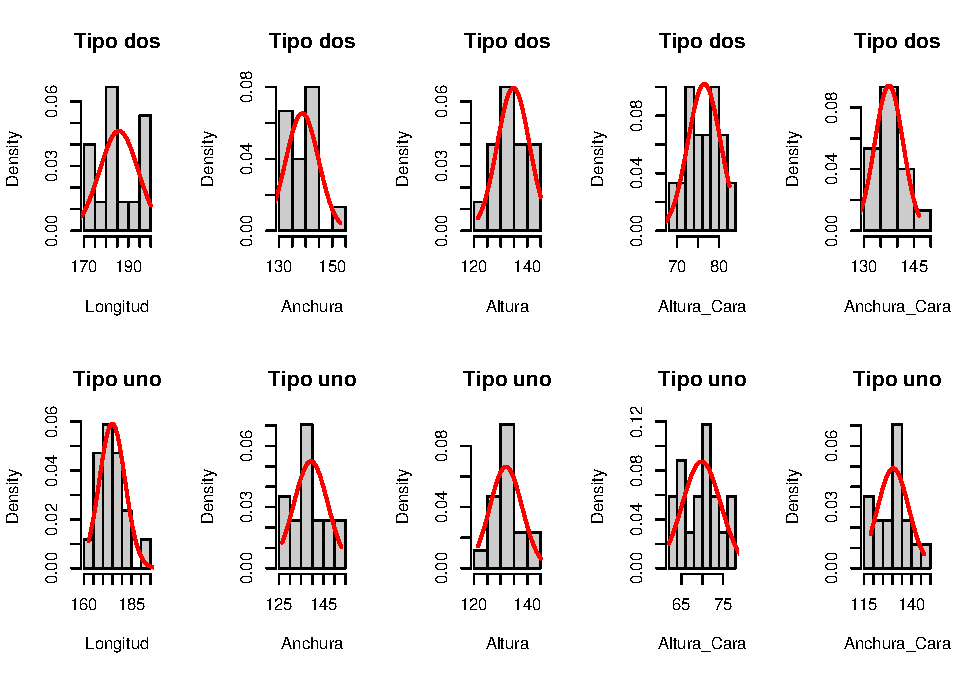
\includegraphics{LDA_files/figure-beamer/unnamed-chunk-7-1.pdf}

\end{frame}

\begin{frame}[fragile]{Normalidad univariante}

\begin{Shaded}
\begin{Highlighting}[]
\CommentTok{# Representación de cuantiles normales de cada variable para cada tipo}

\KeywordTok{par}\NormalTok{(}\DataTypeTok{mfcol =} \KeywordTok{c}\NormalTok{(}\DecValTok{2}\NormalTok{, }\DecValTok{5}\NormalTok{))}
\ControlFlowTok{for}\NormalTok{ (k }\ControlFlowTok{in} \DecValTok{1}\OperatorTok{:}\DecValTok{5}\NormalTok{) \{}
\NormalTok{  j0 <-}\StringTok{ }\KeywordTok{names}\NormalTok{(craneo)[k]}
\NormalTok{  x0 <-}\StringTok{ }\KeywordTok{seq}\NormalTok{(}\KeywordTok{min}\NormalTok{(craneo[, k]), }\KeywordTok{max}\NormalTok{(craneo[, k]), }\DataTypeTok{le =} \DecValTok{1000}\NormalTok{)}
  \ControlFlowTok{for}\NormalTok{ (i }\ControlFlowTok{in} \DecValTok{1}\OperatorTok{:}\DecValTok{2}\NormalTok{) \{}
\NormalTok{    i0 <-}\StringTok{ }\KeywordTok{levels}\NormalTok{(craneo}\OperatorTok{$}\NormalTok{Tipo)[i]}
\NormalTok{    x <-}\StringTok{ }\NormalTok{craneo[craneo}\OperatorTok{$}\NormalTok{Tipo }\OperatorTok{==}\StringTok{ }\NormalTok{i0, j0]}
    \KeywordTok{qqnorm}\NormalTok{(x, }\DataTypeTok{main =} \KeywordTok{paste}\NormalTok{(}\StringTok{"Tipo"}\NormalTok{, i0, j0), }\DataTypeTok{pch =} \DecValTok{19}\NormalTok{, }\DataTypeTok{col =}\NormalTok{ i }\OperatorTok{+}\StringTok{ }\DecValTok{1}\NormalTok{)}
    \KeywordTok{qqline}\NormalTok{(x)}
\NormalTok{  \}}
\NormalTok{\}}
\KeywordTok{par}\NormalTok{(}\DataTypeTok{mfcol =} \KeywordTok{c}\NormalTok{(}\DecValTok{1}\NormalTok{, }\DecValTok{1}\NormalTok{))}
\end{Highlighting}
\end{Shaded}

\end{frame}

\begin{frame}{Normalidad univariante}

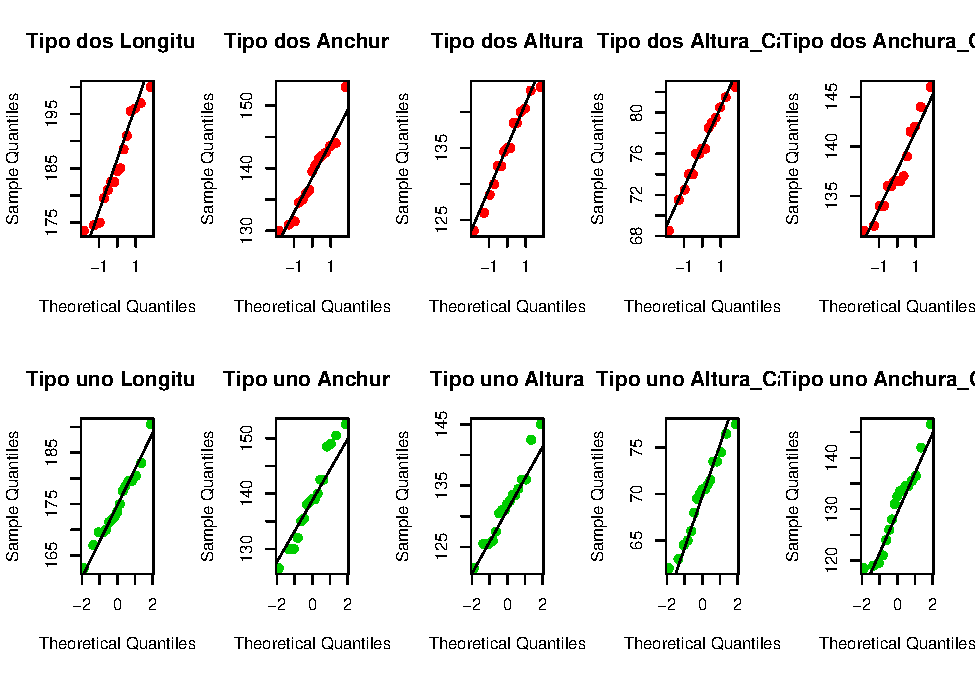
\includegraphics{LDA_files/figure-beamer/unnamed-chunk-8-1.pdf}

\end{frame}

\begin{frame}[fragile]{Normalidad univariante}

\(H_0:\) El conjunto de datos sigue una distribución normal

\(H_1:\) El conjunto de datos no sigue una distribución normal

\begin{Shaded}
\begin{Highlighting}[]
\CommentTok{# Contraste de normalidad Shapiro-Wilk para cada variable en cada tipo de raza}
\KeywordTok{library}\NormalTok{(reshape2)}
\KeywordTok{library}\NormalTok{(knitr)}
\KeywordTok{library}\NormalTok{(dplyr)}
\NormalTok{datos_tidy <-}\StringTok{ }\KeywordTok{melt}\NormalTok{(craneo, }\DataTypeTok{value.name =} \StringTok{"valor"}\NormalTok{)}
\KeywordTok{kable}\NormalTok{(datos_tidy }\OperatorTok\StringTok{ }\KeywordTok{group_by}\NormalTok{(Tipo, variable) }\OperatorTok\StringTok{ }\KeywordTok{summarise}\NormalTok{(}\DataTypeTok{p_value_Shapiro.test =} \KeywordTok{shapiro.test}\NormalTok{(valor)}\OperatorTok{$}\NormalTok{p.value))}
\end{Highlighting}
\end{Shaded}

\end{frame}

\begin{frame}{Normalidad univariante}

\begin{tabular}{l|l|r}
\hline
Tipo & variable & p\_value\_Shapiro.test\\
\hline
dos & Longitud & 0.4003952\\
\hline
dos & Anchura & 0.4665877\\
\hline
dos & Altura & 0.7850492\\
\hline
dos & Altura\_Cara & 0.9395995\\
\hline
dos & Anchura\_Cara & 0.3219514\\
\hline
uno & Longitud & 0.8900856\\
\hline
uno & Anchura & 0.6468092\\
\hline
uno & Altura & 0.6053364\\
\hline
uno & Altura\_Cara & 0.7798472\\
\hline
uno & Anchura\_Cara & 0.4071086\\
\hline
\end{tabular}

\(H_0:\) El conjunto de datos sigue una distribución normal

\(H_1:\) El conjunto de datos no sigue una distribución normal

\end{frame}

\begin{frame}[fragile]{Normalidad univariante}

\hypertarget{left}{}
\begin{verbatim}
##    Tipo     variable     valor
## 1   dos     Longitud 0.4003952
## 2   uno     Longitud 0.8900856
## 3   dos      Anchura 0.4665877
## 4   uno      Anchura 0.6468092
## 5   dos       Altura 0.7850492
## 6   uno       Altura 0.6053364
## 7   dos  Altura_Cara 0.9395995
## 8   uno  Altura_Cara 0.7798472
## 9   dos Anchura_Cara 0.3219514
## 10  uno Anchura_Cara 0.4071086
\end{verbatim}

\hypertarget{right}{}
\begin{Shaded}
\begin{Highlighting}[]
\CommentTok{# Misma operación con aggregate}
\KeywordTok{aggregate}\NormalTok{(}\DataTypeTok{formula =}\NormalTok{ valor }\OperatorTok{~}\StringTok{ }\NormalTok{Tipo }\OperatorTok{+}\StringTok{ }\NormalTok{variable, }\DataTypeTok{data =}\NormalTok{ datos_tidy,}
          \DataTypeTok{FUN =} \ControlFlowTok{function}\NormalTok{(x)\{}\KeywordTok{shapiro.test}\NormalTok{(x)}\OperatorTok{$}\NormalTok{p.value\})}
\end{Highlighting}
\end{Shaded}

\(H_0:\) El conjunto de datos sigue una distribución normal

\(H_1:\) El conjunto de datos no sigue una distribución normal

No hay evidencias de falta de normalidad univariante en ninguna de las
variables empleadas como predictores en ninguno de los grupos.

\end{frame}

\begin{frame}[fragile]{Normalidad multivariante}

El paquete \texttt{MVN} contiene funciones que permiten realizar los
tres test de hipótesis comúnmente empleados para evaluar la normalidad
multivariante (Mardia, Henze-Zirkler y Royston) y también funciones para
identificar outliers que puedan influenciar en el contraste.

\end{frame}

\begin{frame}[fragile]{Normalidad multivariante}

\hypertarget{left}{}
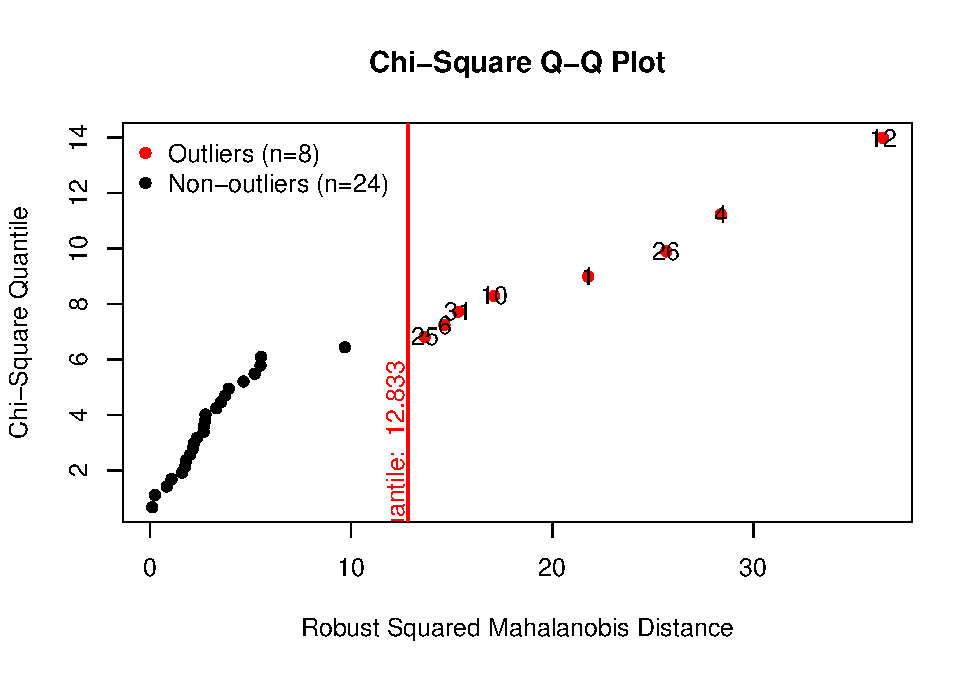
\includegraphics{LDA_files/figure-beamer/unnamed-chunk-11-1.pdf}

\hypertarget{right}{}
\begin{Shaded}
\begin{Highlighting}[]
\KeywordTok{library}\NormalTok{(MVN)}
\NormalTok{outliers <-}\StringTok{ }\KeywordTok{mvn}\NormalTok{(}\DataTypeTok{data =}\NormalTok{ craneo[,}\OperatorTok{-}\DecValTok{6}\NormalTok{], }\DataTypeTok{mvnTest =} \StringTok{"hz"}\NormalTok{, }\DataTypeTok{multivariateOutlierMethod =} \StringTok{"quan"}\NormalTok{)}
\end{Highlighting}
\end{Shaded}

Existen \(n=8\) outliers que podrían influenciar en el contraste de
normalidad multivariante.

\end{frame}

\begin{frame}[fragile]{Normalidad multivariante}

\hypertarget{left}{}
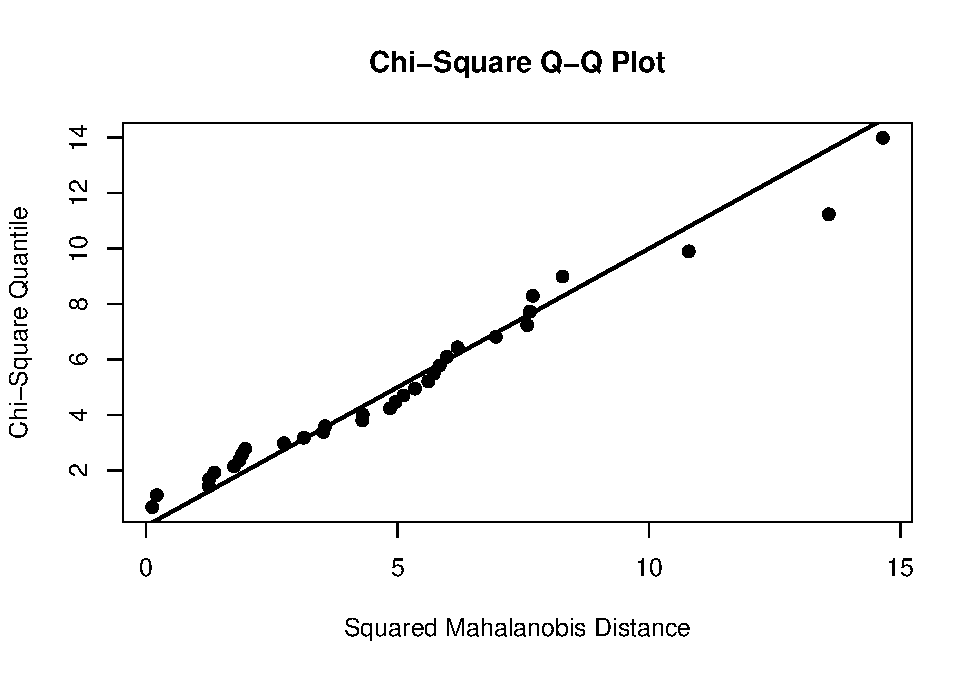
\includegraphics{LDA_files/figure-beamer/unnamed-chunk-12-1.pdf}

\hypertarget{right}{}
\begin{Shaded}
\begin{Highlighting}[]
\NormalTok{royston_test <-}\StringTok{ }\KeywordTok{mvn}\NormalTok{(}\DataTypeTok{data =}\NormalTok{ craneo[,}\OperatorTok{-}\DecValTok{6}\NormalTok{], }\DataTypeTok{mvnTest =} \StringTok{"royston"}\NormalTok{, }\DataTypeTok{multivariatePlot =} \StringTok{"qq"}\NormalTok{)}
\end{Highlighting}
\end{Shaded}

Se pueden apreciar que existen outliers que podrían influenciar en el
contraste de normalidad multivariante.

\end{frame}

\begin{frame}[fragile]{Normalidad multivariante}

\hypertarget{left}{}
\begin{verbatim}
##      Test        H   p value MVN
## 1 Royston 4.942764 0.4233818 YES
\end{verbatim}

\begin{verbatim}
##            Test        HZ   p value MVN
## 1 Henze-Zirkler 0.8261507 0.3755845 YES
\end{verbatim}

\hypertarget{right}{}
\begin{Shaded}
\begin{Highlighting}[]
\NormalTok{royston_test}\OperatorTok{$}\NormalTok{multivariateNormality}
\NormalTok{hz_test <-}\StringTok{ }\KeywordTok{mvn}\NormalTok{(}\DataTypeTok{data =}\NormalTok{ craneo[,}\OperatorTok{-}\DecValTok{6}\NormalTok{], }\DataTypeTok{mvnTest =} \StringTok{"hz"}\NormalTok{)}
\NormalTok{hz_test}\OperatorTok{$}\NormalTok{multivariateNormality}
\end{Highlighting}
\end{Shaded}

\(H_0:\) El conjunto de datos sigue una distribución normal
multivariante

\(H_1:\) El conjunto de datos no sigue una distribución normal
multivariante

A pesar de los \(n=8\) outliers detectados, ninguno de los dos test
encuentran evidencias significativas (\(\alpha=0.05\)) de falta de
normalidad multivariante.

\end{frame}

\begin{frame}{Homogeneidad de Varianza}

El test Box M fue desarrollado por el matemático Box (1949) como una
extensión del test de Barttlet para escenarios multivariante y permite
contrastar la igualdad de matrices entre grupos. El test Box M es muy
sensible a violaciones de la normalidad multivariante, por lo que esta
debe ser contrastada con anterioridad. Ocurre con frecuencia, que el
resultado de un test Box M resulta significativo debido a la falta de
distribución normal multivariante en lugar de por falta de homogeneidad
en las matrices de covarianza. Dada la sensibilidad de este test se
recomienda emplear un límite de significancia de 0.001 (Tabachnick \&
Fidell, 2001, y
\url{http://www.real-statistics.com/multivariate-statistics/}).

\end{frame}

\begin{frame}[fragile]{Homogeneidad de Varianza}

\hypertarget{left}{}
\begin{verbatim}
## 
##  Box's M-test for Homogeneity of Covariance Matrices
## 
## data:  craneo[, 1:5]
## Chi-Sq (approx.) = 18.371, df = 15, p-value = 0.2437
\end{verbatim}

\hypertarget{right}{}
\begin{Shaded}
\begin{Highlighting}[]
\KeywordTok{library}\NormalTok{(biotools)}
\KeywordTok{boxM}\NormalTok{(}\DataTypeTok{data =}\NormalTok{ craneo[, }\DecValTok{1}\OperatorTok{:}\DecValTok{5}\NormalTok{], }\DataTypeTok{grouping =}\NormalTok{ craneo[, }\DecValTok{6}\NormalTok{])}
\end{Highlighting}
\end{Shaded}

\(H_0:\) La matriz de covarianza es igual en todos los grupos

\(H_1:\) La matriz de covarianza no es igual en todos los grupos

La prueba de hipotesis no encuentran evidencias significativas
(\(\alpha=0.05\)) de falta de homogenidad de la matriz de covarianza en
todos los grupos.

\end{frame}

\begin{frame}[fragile]{Análisis discriminante lineal2}

\hypertarget{left}{}
\begin{verbatim}
## Call:
## lda(Tipo ~ Longitud + Anchura + Altura + Altura_Cara + Anchura_Cara, 
##     data = craneo)
## 
## Prior probabilities of groups:
##     dos     uno 
## 0.46875 0.53125 
## 
## Group means:
##     Longitud  Anchura   Altura Altura_Cara Anchura_Cara
## dos 185.7333 138.7333 134.7667    76.46667     137.5000
## uno 174.8235 139.3529 132.0000    69.82353     130.3529
## 
## Coefficients of linear discriminants:
##                       LD1
## Longitud     -0.047726591
## Anchura       0.083247929
## Altura        0.002795841
## Altura_Cara  -0.094695000
## Anchura_Cara -0.094809401
\end{verbatim}

\hypertarget{right}{}
\begin{Shaded}
\begin{Highlighting}[]
\KeywordTok{library}\NormalTok{(MASS)}
\NormalTok{modelo_lda <-}\StringTok{ }\KeywordTok{lda}\NormalTok{(}\DataTypeTok{formula =}\NormalTok{ Tipo }\OperatorTok{~}\StringTok{ }\NormalTok{Longitud }\OperatorTok{+}\StringTok{ }\NormalTok{Anchura }\OperatorTok{+}\StringTok{ }\NormalTok{Altura }\OperatorTok{+}\StringTok{ }\NormalTok{Altura_Cara }\OperatorTok{+}\StringTok{ }\NormalTok{Anchura_Cara, }\DataTypeTok{data =}\NormalTok{ craneo)}
\NormalTok{modelo_lda}
\end{Highlighting}
\end{Shaded}

La función \texttt{lda} del paquete \texttt{MASS}. lda realiza la
clasificación mediante la aproximación de Fisher.

\end{frame}

\begin{frame}[fragile]{Clasificación de nuevos craneos}

\begin{Shaded}
\begin{Highlighting}[]
\NormalTok{nuevosdatos <-}
\StringTok{  }\KeywordTok{rbind}\NormalTok{(}\KeywordTok{c}\NormalTok{(}\DecValTok{171}\NormalTok{,}\FloatTok{140.5}\NormalTok{,}\FloatTok{127.0}\NormalTok{,}\FloatTok{69.5}\NormalTok{,}\FloatTok{137.0}\NormalTok{),}\KeywordTok{c}\NormalTok{(}\FloatTok{179.0}\NormalTok{,}\FloatTok{132.0}\NormalTok{,}\FloatTok{140.0}\NormalTok{,}\FloatTok{72.0}\NormalTok{,}\FloatTok{138.5}\NormalTok{))}
\CommentTok{# Asigno a los dos nuevos datos los nombres de las variables}
\KeywordTok{colnames}\NormalTok{(nuevosdatos) <-}\StringTok{ }\KeywordTok{colnames}\NormalTok{(craneo[,}\OperatorTok{-}\DecValTok{6}\NormalTok{])}
\NormalTok{nuevosdatos <-}\StringTok{ }\KeywordTok{data.frame}\NormalTok{(nuevosdatos)}
\NormalTok{nuevosdatos}
\CommentTok{# Se predice el grupo de pertenencia de los nuevos datos}
\KeywordTok{predict}\NormalTok{(modelo_lda,}\DataTypeTok{newdata=}\NormalTok{nuevosdatos)}\OperatorTok{$}\NormalTok{class}
\KeywordTok{predict}\NormalTok{(modelo_lda,}\DataTypeTok{newdata=}\NormalTok{nuevosdatos)}
\end{Highlighting}
\end{Shaded}

\end{frame}

\begin{frame}[fragile]{Clasificación de nuevos craneos}

\hypertarget{left}{}
\begin{verbatim}
##   Longitud Anchura Altura Altura_Cara Anchura_Cara
## 1      171   140.5    127        69.5        137.0
## 2      179   132.0    140        72.0        138.5
\end{verbatim}

\begin{verbatim}
## [1] uno dos
## Levels: dos uno
\end{verbatim}

\begin{verbatim}
## $class
## [1] uno dos
## Levels: dos uno
## 
## $posterior
##         dos       uno
## 1 0.2230540 0.7769460
## 2 0.8071613 0.1928387
## 
## $x
##          LD1
## 1  0.5415596
## 2 -0.8904662
\end{verbatim}

\hypertarget{right}{}
Por ejemplo, dos nuevos craneos cuyas medidas sean: Longitud=171,
Anchura=140.5, Altura=127, Altura\_Cara=69.5, y Anchura\_Cara=137.
Longitud=179, Anchura=132, Altura=140, Altura\_Cara=72, y
Anchura\_Cara=138.5. La probabilidad posterior de que el primer craneo
pertenezca a la raza tipo 1 es del 77.69\% frente al 22.31\% de que
pertenezca a la raza tipo 2. La probabilidad posterior de que el segundo
craneo pertenezca a la raza tipo 1 es del 19.28\% frente al 80.72\% de
que pertenezca a la raza tipo 2.

\end{frame}

\begin{frame}[fragile]{Evaluación de los errores de clasificación}

\hypertarget{left}{}
\begin{verbatim}
##           Clase predicha
## Clase real dos uno
##        dos  11   4
##        uno   3  14
\end{verbatim}

\begin{verbatim}
## [1] "trainig_error= 21.875 %"
\end{verbatim}

Empleando las mismas observaciones con las que se ha generado el modelo
discriminante (trainig data), la precisión de clasificación es del
78.13\%. Evaluar un modelo con los mismos datos con los que se ha creado
suele resultar en estimaciones de la precisión demasiado optimistas
(training error muy bajo).

\hypertarget{right}{}
\begin{Shaded}
\begin{Highlighting}[]
\NormalTok{predicciones <-}\StringTok{ }\KeywordTok{predict}\NormalTok{(}\DataTypeTok{object =}\NormalTok{ modelo_lda, }\DataTypeTok{newdata =}\NormalTok{ craneo[, }\OperatorTok{-}\DecValTok{6}\NormalTok{],}
                        \DataTypeTok{method =} \StringTok{"predictive"}\NormalTok{)}
\KeywordTok{table}\NormalTok{(craneo}\OperatorTok{$}\NormalTok{Tipo, predicciones}\OperatorTok{$}\NormalTok{class,}
      \DataTypeTok{dnn =} \KeywordTok{c}\NormalTok{(}\StringTok{"Clase real"}\NormalTok{, }\StringTok{"Clase predicha"}\NormalTok{))}

\NormalTok{trainig_error <-}\StringTok{ }\KeywordTok{mean}\NormalTok{(craneo}\OperatorTok{$}\NormalTok{Tipo }\OperatorTok{!=}\StringTok{ }\NormalTok{predicciones}\OperatorTok{$}\NormalTok{class) }\OperatorTok{*}\StringTok{ }\DecValTok{100}
\KeywordTok{paste}\NormalTok{(}\StringTok{"trainig_error="}\NormalTok{, trainig_error, }\StringTok{"%"}\NormalTok{)}
\end{Highlighting}
\end{Shaded}

\end{frame}

\begin{frame}[fragile]{Visualización de las clasificaciones}

\begin{Shaded}
\begin{Highlighting}[]
\KeywordTok{library}\NormalTok{(klaR)}
\KeywordTok{partimat}\NormalTok{(Tipo }\OperatorTok{~}\StringTok{ }\NormalTok{Longitud }\OperatorTok{+}\StringTok{ }\NormalTok{Anchura }\OperatorTok{+}\StringTok{ }\NormalTok{Altura }\OperatorTok{+}\StringTok{ }\NormalTok{Altura_Cara }\OperatorTok{+}\StringTok{ }\NormalTok{Anchura_Cara,}\DataTypeTok{data=}\NormalTok{craneo, }\DataTypeTok{method =} \StringTok{"lda"}\NormalTok{, }\DataTypeTok{prec =} \DecValTok{200}\NormalTok{,}
         \DataTypeTok{image.colors =} \KeywordTok{c}\NormalTok{(}\StringTok{"darkgoldenrod1"}\NormalTok{, }\StringTok{"skyblue2"}\NormalTok{),}
         \DataTypeTok{col.mean =} \StringTok{"firebrick"}\NormalTok{)}
\end{Highlighting}
\end{Shaded}

\end{frame}

\begin{frame}{Visualización de las clasificaciones}

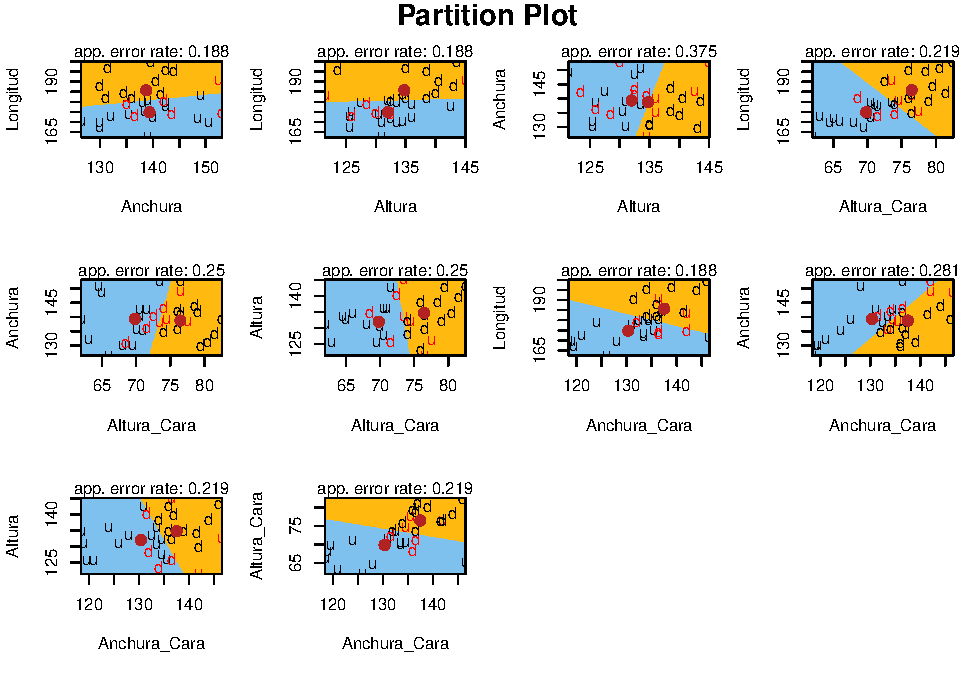
\includegraphics{LDA_files/figure-beamer/unnamed-chunk-18-1.pdf}

Se desea predecir si un paciente pertenece a una de las siguientes cla-
ses: Normal (el paciente esta sano), Chemical (el paciente presenta
pre-diabetes) y Overt (el paciente presenta diabetes) utilizando tres
indicadores de la sangre (glucosa,insulina y sspg).

\end{frame}

\begin{frame}[fragile]{Ejemplo 2}

Se desea predecir si un paciente pertenece a una de las siguientes
clases: \texttt{Normal} (el paciente esta sano), \texttt{Chemical} (el
paciente presenta pre-diabetes) y \texttt{Overt} (el paciente presenta
diabetes) utilizando tres indicadores de la sangre (glucosa,insulina y
sspg).

\end{frame}

\begin{frame}[fragile]{cargando el conjunto de datos}

\begin{Shaded}
\begin{Highlighting}[]
\NormalTok{diabetes=}\KeywordTok{read.csv}\NormalTok{(}\StringTok{"DiabetesTrain.csv"}\NormalTok{)}
\NormalTok{diabetes}
\end{Highlighting}
\end{Shaded}

\begin{verbatim}
##     glucose insulin sspg    class
## 1        97     289  117   normal
## 2       105     319  143   normal
## 3        90     356  199   normal
## 4        90     323  240   normal
## 5        86     381  157   normal
## 6       100     350  221   normal
## 7        85     301  186   normal
## 8        97     379  142   normal
## 9        97     296  131   normal
## 10       91     353  221   normal
## 11       87     306  178   normal
## 12       78     290  136   normal
## 13       90     371  200   normal
## 14       80     393  202   normal
## 15       90     364  152   normal
## 16       99     359  185   normal
## 17       85     296  116   normal
## 18       90     345  123   normal
## 19       90     378  136   normal
## 20       88     304  134   normal
## 21       90     327  192   normal
## 22       92     386  279   normal
## 23       98     365  145   normal
## 24      100     352  172   normal
## 25       86     325  179   normal
## 26       98     321  222   normal
## 27       70     360  134   normal
## 28       99     336  143   normal
## 29       75     352  169   normal
## 30       90     353  263   normal
## 31       85     373  174   normal
## 32       99     376  134   normal
## 33      100     367  182   normal
## 34       78     335  241   normal
## 35      106     396  128   normal
## 36      102     378  165   normal
## 37       90     360  282   normal
## 38       94     291   94   normal
## 39       80     269  121   normal
## 40       93     318   73   normal
## 41       96     356  112   normal
## 42       88     291  157   normal
## 43       94     313  200   normal
## 44       93     306  220   normal
## 45       86     319  144   normal
## 46       96     332  151   normal
## 47       86     323  158   normal
## 48       89     323   73   normal
## 49       83     351   81   normal
## 50       98     478  151 chemical
## 51      100     398  122   normal
## 52      110     426  117   normal
## 53       88     439  208 chemical
## 54       80     333  131   normal
## 55       91     436  148 chemical
## 56       96     418  130   normal
## 57       95     391  137   normal
## 58       84     416  146   normal
## 59      100     385  192   normal
## 60       86     393  115   normal
## 61       93     376  195   normal
## 62      107     403  267   normal
## 63      112     414  281   normal
## 64       94     426  213 chemical
## 65       93     364  156   normal
## 66       93     391  221   normal
## 67       90     356  199   normal
## 68       99     398   76   normal
## 69       93     393  490   normal
## 70       85     425  143 chemical
## 71       89     318   73   normal
## 72      111     558  748 chemical
## 73      114     540  188 chemical
## 74      101     469  607 chemical
## 75      112     568  232 chemical
## 76      105     527  480 chemical
## 77      103     537  622 chemical
## 78       99     466  287 chemical
## 79      102     599  266 chemical
## 80       96     456  326 chemical
## 81       95     517  564 chemical
## 82      110     522  325 chemical
## 83       92     476  433 chemical
## 84      104     472  180 chemical
## 85       92     442  109 chemical
## 86       92     541  313 chemical
## 87       92     580  132 chemical
## 88       93     472  285 chemical
## 89      112     562  139 chemical
## 90       88     423  212 chemical
## 91      114     643  155 chemical
## 92      103     533  120 chemical
## 93      303    1487   23    overt
## 94      125     714  232    overt
## 95      280    1470   54    overt
## 96      216    1113   81    overt
## 97      190     972   87    overt
## 98      303    1364   42    overt
## 99      173     832  102    overt
## 100     203     967  138    overt
## 101     140     613  131    overt
## 102     275    1373   45    overt
## 103     260    1133  118    overt
## 104     233    1183   73    overt
## 105     146     847  103    overt
## 106     124     538  460    overt
## 107     213    1001   42    overt
## 108     330    1520   13    overt
## 109     123     557  130    overt
## 110     130     670   44    overt
## 111     120     636  314    overt
## 112     138     741  219    overt
## 113     188     958  100    overt
## 114     339    1354   10    overt
## 115     213    1025   29    overt
\end{verbatim}

\end{frame}

\begin{frame}[fragile]{Exploración gráfica de los datos}

\begin{Shaded}
\begin{Highlighting}[]
\KeywordTok{library}\NormalTok{(ggplot2)}
\KeywordTok{library}\NormalTok{(ggpubr)}

\NormalTok{plot1 <-}\StringTok{ }\KeywordTok{ggplot}\NormalTok{(}\DataTypeTok{data =}\NormalTok{ diabetes, }\KeywordTok{aes}\NormalTok{(}\DataTypeTok{x =}\NormalTok{ glucose)) }\OperatorTok{+}
\StringTok{  }\KeywordTok{geom_density}\NormalTok{(}\KeywordTok{aes}\NormalTok{(}\DataTypeTok{colour =}\NormalTok{ class)) }\OperatorTok{+}\StringTok{ }\KeywordTok{theme_bw}\NormalTok{()}
\NormalTok{plot2 <-}\StringTok{ }\KeywordTok{ggplot}\NormalTok{(}\DataTypeTok{data =}\NormalTok{ diabetes, }\KeywordTok{aes}\NormalTok{(}\DataTypeTok{x =}\NormalTok{ insulin)) }\OperatorTok{+}
\StringTok{  }\KeywordTok{geom_density}\NormalTok{(}\KeywordTok{aes}\NormalTok{(}\DataTypeTok{colour =}\NormalTok{ class)) }\OperatorTok{+}\StringTok{ }\KeywordTok{theme_bw}\NormalTok{()}
\NormalTok{plot3 <-}\StringTok{ }\KeywordTok{ggplot}\NormalTok{(}\DataTypeTok{data =}\NormalTok{ diabetes, }\KeywordTok{aes}\NormalTok{(}\DataTypeTok{x =}\NormalTok{ sspg)) }\OperatorTok{+}
\StringTok{  }\KeywordTok{geom_density}\NormalTok{(}\KeywordTok{aes}\NormalTok{(}\DataTypeTok{colour =}\NormalTok{ class)) }\OperatorTok{+}\StringTok{ }\KeywordTok{theme_bw}\NormalTok{()}
\CommentTok{# la función grid.arrange del paquete grid.extra permite ordenar}
\CommentTok{# graficos de ggplot2}
\KeywordTok{ggarrange}\NormalTok{(plot1, plot2, plot3, }\DataTypeTok{common.legend =} \OtherTok{TRUE}\NormalTok{, }\DataTypeTok{legend =} \StringTok{"bottom"}\NormalTok{)}
\end{Highlighting}
\end{Shaded}

\end{frame}

\begin{frame}{Exploración gráfica de los datos}

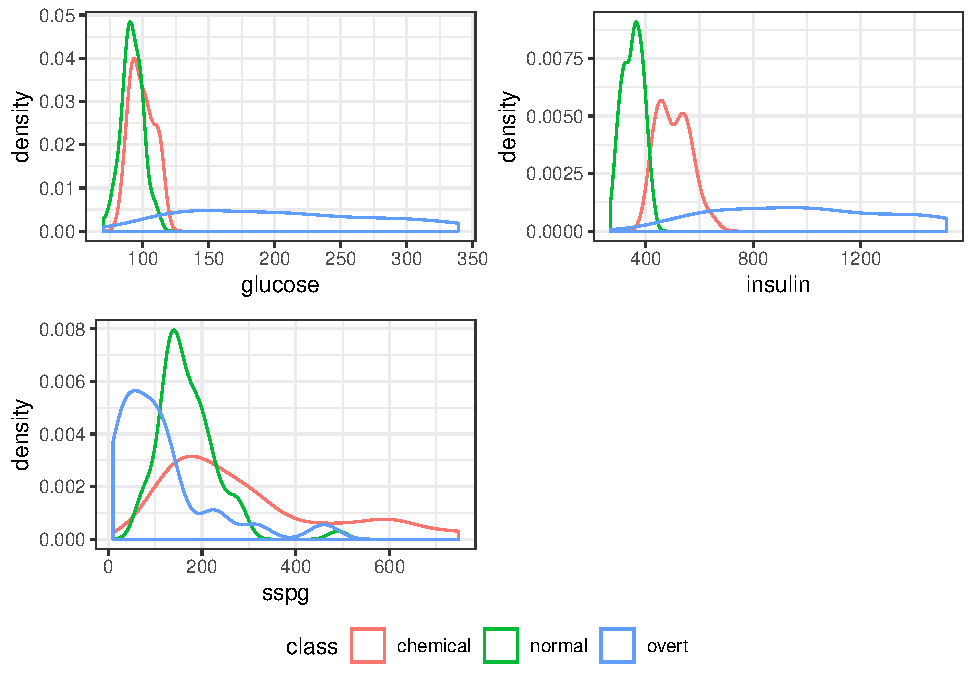
\includegraphics{LDA_files/figure-beamer/unnamed-chunk-20-1.pdf}

\end{frame}

\begin{frame}{Exploración gráfica de los datos}

\hypertarget{left}{}
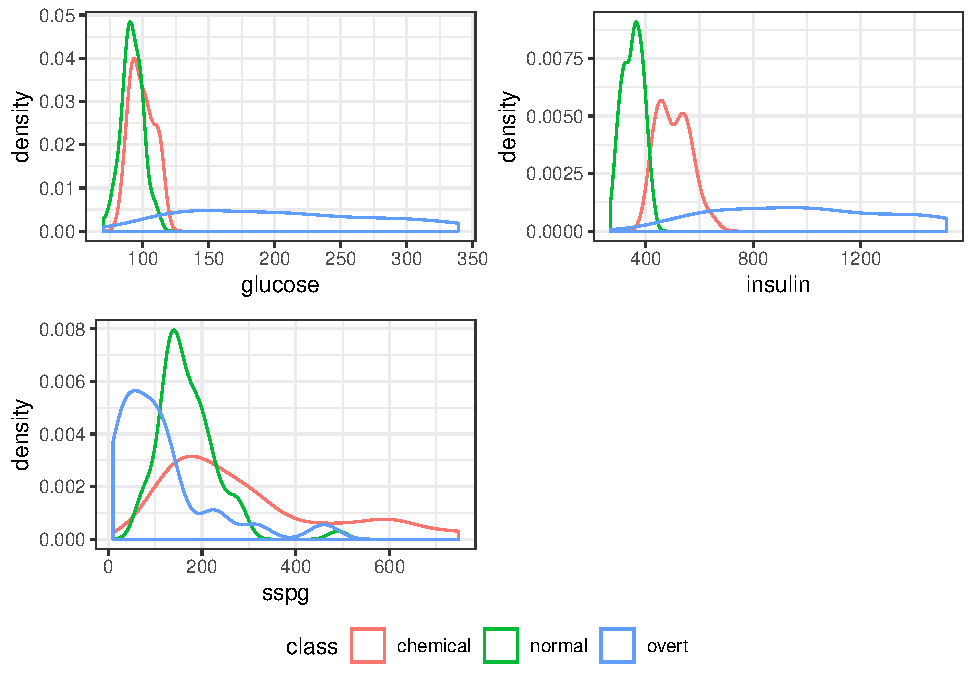
\includegraphics{LDA_files/figure-beamer/unnamed-chunk-21-1.pdf}

\hypertarget{right}{}
La variable sspg presenta asimetría positiva dentro de cada grupo de
pacientes.

\end{frame}

\begin{frame}{Exploración gráfica de los datos}

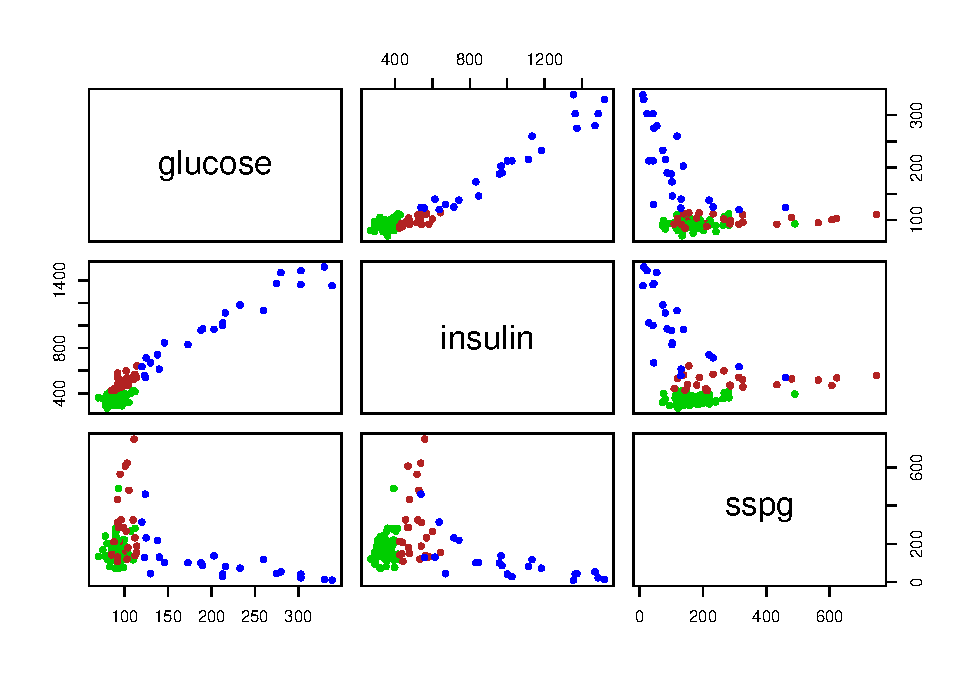
\includegraphics{LDA_files/figure-beamer/unnamed-chunk-22-1.pdf}

\end{frame}

\begin{frame}[fragile]{Exploración gráfica de los datos}

\hypertarget{left}{}
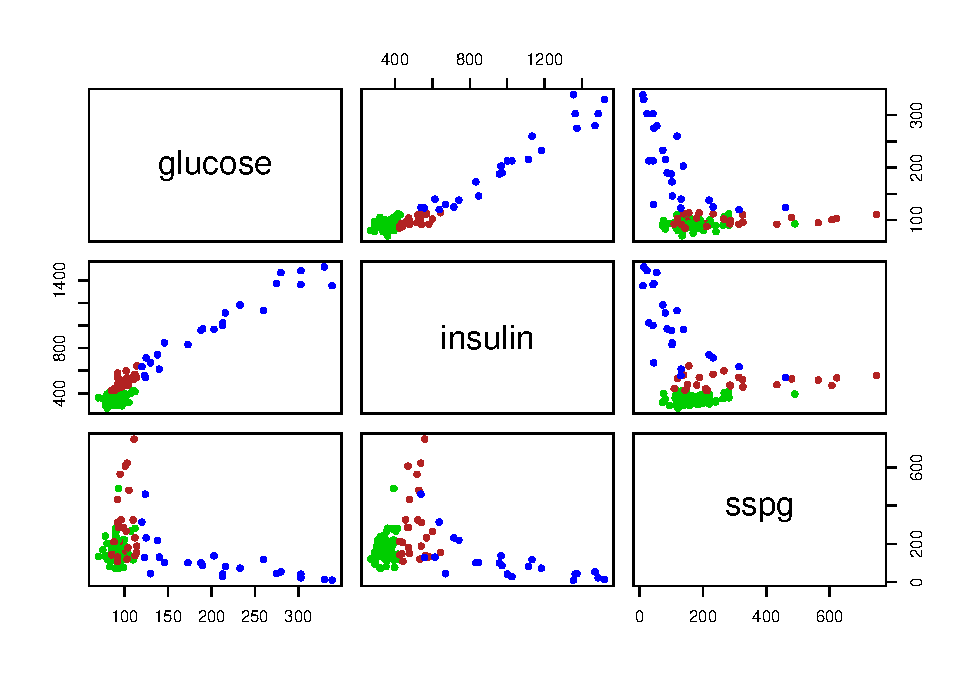
\includegraphics{LDA_files/figure-beamer/unnamed-chunk-23-1.pdf}

\hypertarget{right}{}
\begin{Shaded}
\begin{Highlighting}[]
\KeywordTok{pairs}\NormalTok{(}\DataTypeTok{x =}\NormalTok{ diabetes[, }\OperatorTok{-}\DecValTok{4}\NormalTok{], }\DataTypeTok{col =} \KeywordTok{c}\NormalTok{(}\StringTok{"firebrick"}\NormalTok{, }\StringTok{"green3"}\NormalTok{, }\StringTok{"blue"}\NormalTok{)[diabetes}\OperatorTok{$}\NormalTok{class],}
      \DataTypeTok{pch =} \DecValTok{20}\NormalTok{)}
\end{Highlighting}
\end{Shaded}

Las variables glucosa e insulina son las dos variables con más potencial
para poder separar entre clases de pacientes. Sin embargo, están
altamente correlacionadas, por lo que la información que aportan es en
gran medida redundante.

\end{frame}

\begin{frame}[fragile]{Probabilidades a priori}

Como no se dispone de información sobre la abundancia relativa de las
clases de pacientes a nivel poblacional, se considera como probabilidad
previa de cada clase el número de observaciones por clase de paciente
entre el número de observaciones totales.

\begin{Shaded}
\begin{Highlighting}[]
\KeywordTok{table}\NormalTok{(diabetes[,}\DecValTok{4}\NormalTok{])}\OperatorTok{/}\KeywordTok{nrow}\NormalTok{(diabetes)}
\end{Highlighting}
\end{Shaded}

\begin{verbatim}
## 
## chemical   normal    overt 
## 0.226087 0.573913 0.200000
\end{verbatim}

\[\hat{\pi}_{sano}=0.57\text{,} \quad \hat{\pi}_{pre}=0.23 \quad \text{y} \quad \hat{\pi}_{diab}=0.20\]

\end{frame}

\begin{frame}[fragile]{Normalidad univariante}

\begin{Shaded}
\begin{Highlighting}[]
\CommentTok{#representación mediante histograma de cada variable para cada clase}

\KeywordTok{par}\NormalTok{(}\DataTypeTok{mar =} \KeywordTok{rep}\NormalTok{(}\DecValTok{3}\NormalTok{, }\DecValTok{3}\NormalTok{))}
\ControlFlowTok{for}\NormalTok{ (k }\ControlFlowTok{in} \DecValTok{1}\OperatorTok{:}\DecValTok{3}\NormalTok{) \{}
\NormalTok{  j0 <-}\StringTok{ }\KeywordTok{names}\NormalTok{(diabetes)[k]}
\NormalTok{  x0 <-}\StringTok{ }\KeywordTok{seq}\NormalTok{(}\KeywordTok{min}\NormalTok{(diabetes[, k]), }\KeywordTok{max}\NormalTok{(diabetes[, k]), }\DataTypeTok{le =} \DecValTok{1000}\NormalTok{)}
  \ControlFlowTok{for}\NormalTok{ (i }\ControlFlowTok{in} \DecValTok{1}\OperatorTok{:}\DecValTok{3}\NormalTok{) \{}
\NormalTok{    i0 <-}\StringTok{ }\KeywordTok{levels}\NormalTok{(diabetes}\OperatorTok{$}\NormalTok{class)[i]}
\NormalTok{    x <-}\StringTok{ }\NormalTok{diabetes[diabetes}\OperatorTok{$}\NormalTok{class }\OperatorTok{==}\StringTok{ }\NormalTok{i0, j0]}
    \KeywordTok{hist}\NormalTok{(x, }\DataTypeTok{proba =}\NormalTok{ T, }\DataTypeTok{col =} \KeywordTok{grey}\NormalTok{(}\FloatTok{0.8}\NormalTok{), }\DataTypeTok{main =} \KeywordTok{paste}\NormalTok{(}\StringTok{"class"}\NormalTok{, i0),}
         \DataTypeTok{xlab =}\NormalTok{ j0)}
    \KeywordTok{lines}\NormalTok{(x0, }\KeywordTok{dnorm}\NormalTok{(x0, }\KeywordTok{mean}\NormalTok{(x), }\KeywordTok{sd}\NormalTok{(x)), }\DataTypeTok{col =} \StringTok{"red"}\NormalTok{, }\DataTypeTok{lwd =} \DecValTok{2}\NormalTok{)}
\NormalTok{  \}}
\NormalTok{\}}
\KeywordTok{par}\NormalTok{(}\DataTypeTok{mar =} \KeywordTok{rep}\NormalTok{(}\DecValTok{1}\NormalTok{, }\DecValTok{1}\NormalTok{))}
\end{Highlighting}
\end{Shaded}

\end{frame}

\begin{frame}{Normalidad univariante}

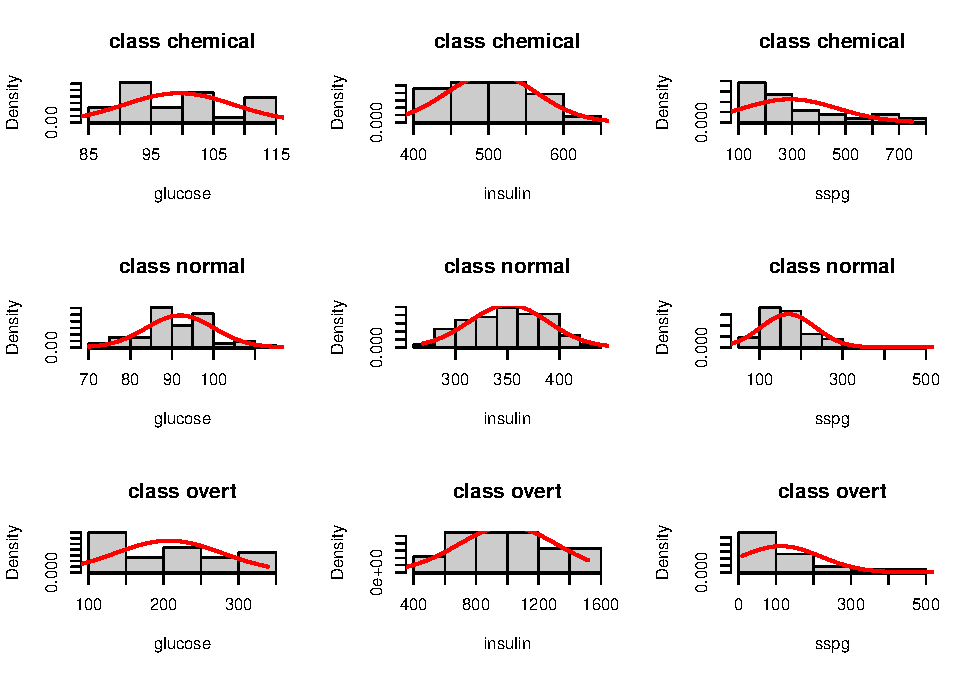
\includegraphics{LDA_files/figure-beamer/unnamed-chunk-25-1.pdf}

\end{frame}

\begin{frame}[fragile]{Normalidad univariante}

\begin{Shaded}
\begin{Highlighting}[]
\CommentTok{#representación de cuantiles normales de cada variable para cada clase}

\KeywordTok{par}\NormalTok{(}\DataTypeTok{mfcol =} \KeywordTok{c}\NormalTok{(}\DecValTok{3}\NormalTok{, }\DecValTok{3}\NormalTok{))}
\ControlFlowTok{for}\NormalTok{ (k }\ControlFlowTok{in} \DecValTok{1}\OperatorTok{:}\DecValTok{3}\NormalTok{) \{}
\NormalTok{  j0 <-}\StringTok{ }\KeywordTok{names}\NormalTok{(diabetes)[k]}
\NormalTok{  x0 <-}\StringTok{ }\KeywordTok{seq}\NormalTok{(}\KeywordTok{min}\NormalTok{(diabetes[, k]), }\KeywordTok{max}\NormalTok{(diabetes[, k]), }\DataTypeTok{le =} \DecValTok{1000}\NormalTok{)}
  \ControlFlowTok{for}\NormalTok{ (i }\ControlFlowTok{in} \DecValTok{1}\OperatorTok{:}\DecValTok{3}\NormalTok{) \{}
\NormalTok{    i0 <-}\StringTok{ }\KeywordTok{levels}\NormalTok{(diabetes}\OperatorTok{$}\NormalTok{class)[i]}
\NormalTok{    x <-}\StringTok{ }\NormalTok{diabetes[diabetes}\OperatorTok{$}\NormalTok{class }\OperatorTok{==}\StringTok{ }\NormalTok{i0, j0]}
    \KeywordTok{qqnorm}\NormalTok{(x, }\DataTypeTok{main =} \KeywordTok{paste}\NormalTok{(i0, j0), }\DataTypeTok{pch =} \DecValTok{19}\NormalTok{, }\DataTypeTok{col =}\NormalTok{ i }\OperatorTok{+}\StringTok{ }\DecValTok{1}\NormalTok{) }
    \KeywordTok{qqline}\NormalTok{(x)}
\NormalTok{  \}}
\NormalTok{\}}
\KeywordTok{par}\NormalTok{(}\DataTypeTok{mfcol =} \KeywordTok{c}\NormalTok{(}\DecValTok{1}\NormalTok{, }\DecValTok{1}\NormalTok{))}
\end{Highlighting}
\end{Shaded}

\end{frame}

\begin{frame}{Normalidad univariante}

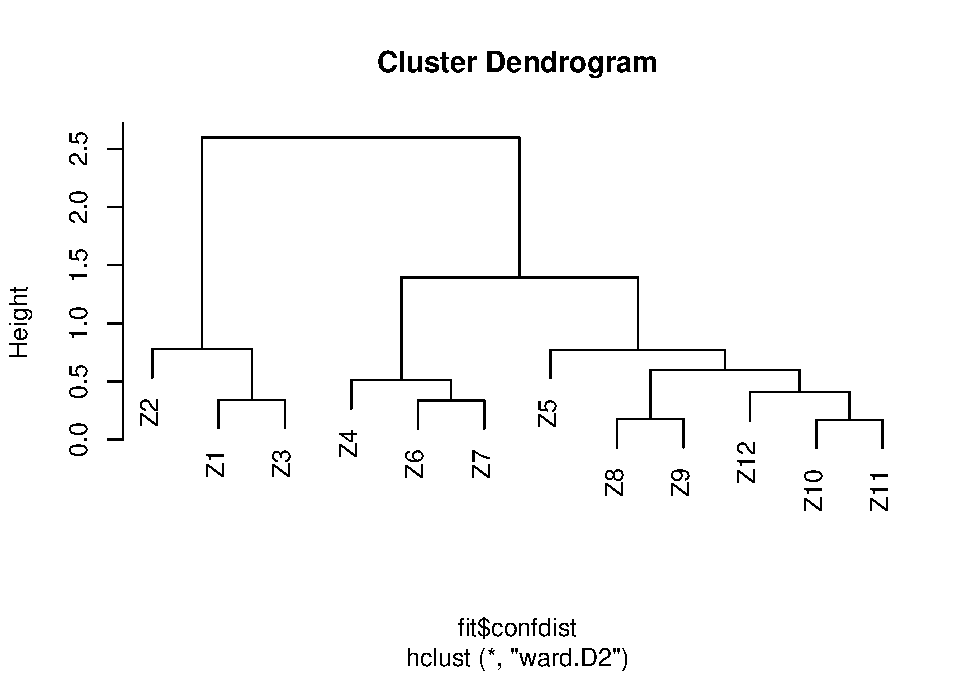
\includegraphics{LDA_files/figure-beamer/unnamed-chunk-26-1.pdf}

\end{frame}

\begin{frame}[fragile]{Normalidad univariante}

\(H_0:\) El conjunto de datos sigue una distribución normal

\(H_1:\) El conjunto de datos no sigue una distribución normal

\begin{Shaded}
\begin{Highlighting}[]
\CommentTok{# Contraste de normalidad Shapiro-Wilk para cada variable en cada clase}
\KeywordTok{library}\NormalTok{(reshape2)}
\KeywordTok{library}\NormalTok{(knitr)}
\KeywordTok{library}\NormalTok{(dplyr)}
\NormalTok{datos_tidy <-}\StringTok{ }\KeywordTok{melt}\NormalTok{(diabetes, }\DataTypeTok{value.name =} \StringTok{"valor"}\NormalTok{)}
\KeywordTok{kable}\NormalTok{(datos_tidy }\OperatorTok\StringTok{ }\KeywordTok{group_by}\NormalTok{(class, variable) }\OperatorTok\StringTok{ }\KeywordTok{summarise}\NormalTok{(}\DataTypeTok{p_value_Shapiro.test =} \KeywordTok{round}\NormalTok{(}\KeywordTok{shapiro.test}\NormalTok{(valor)}\OperatorTok{$}\NormalTok{p.value,}\DecValTok{5}\NormalTok{)))}

\end{Highlighting}
\end{Shaded}

\end{frame}

\begin{frame}{Normalidad univariante}

\begin{tabular}{l|l|r}
\hline
class & variable & p\_value\_Shapiro.test\\
\hline
chemical & glucose & 0.11551\\
\hline
chemical & insulin & 0.17119\\
\hline
chemical & sspg & 0.00133\\
\hline
normal & glucose & 0.81720\\
\hline
normal & insulin & 0.26450\\
\hline
normal & sspg & 0.00000\\
\hline
overt & glucose & 0.05406\\
\hline
overt & insulin & 0.18050\\
\hline
overt & sspg & 0.00031\\
\hline
\end{tabular}

\(H_0:\) El conjunto de datos sigue una distribución normal

\(H_1:\) El conjunto de datos no sigue una distribución normal

\end{frame}

\begin{frame}[fragile]{Normalidad multivariante}

\hypertarget{left}{}
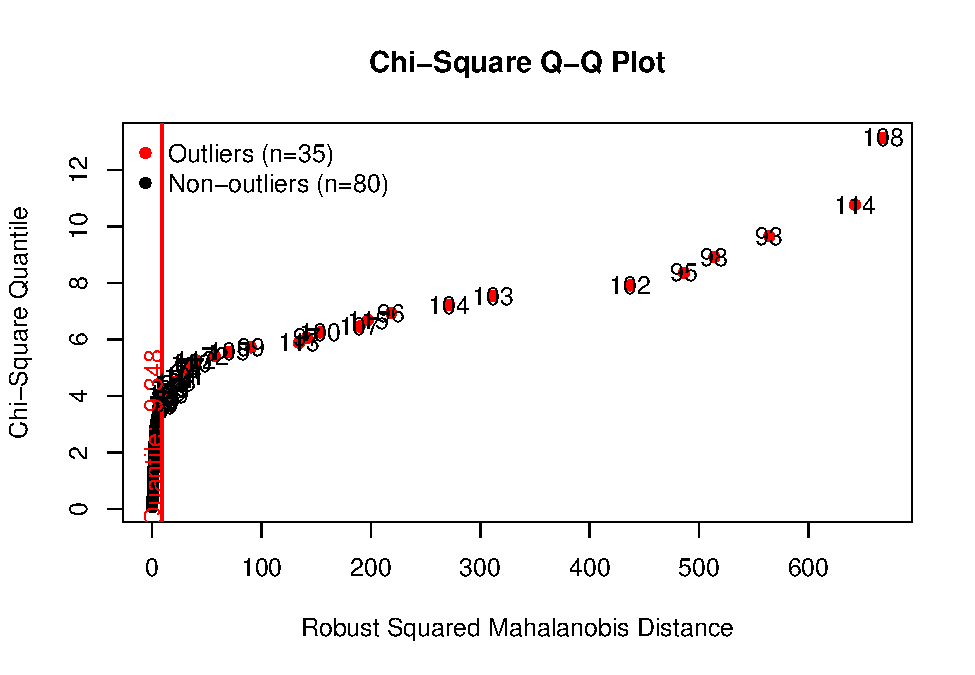
\includegraphics{LDA_files/figure-beamer/unnamed-chunk-28-1.pdf}

\hypertarget{right}{}
\begin{Shaded}
\begin{Highlighting}[]
\KeywordTok{library}\NormalTok{(MVN)}
\NormalTok{outliers <-}\StringTok{ }\KeywordTok{mvn}\NormalTok{(}\DataTypeTok{data =}\NormalTok{ diabetes[,}\OperatorTok{-}\DecValTok{4}\NormalTok{], }\DataTypeTok{mvnTest =} \StringTok{"hz"}\NormalTok{, }\DataTypeTok{multivariateOutlierMethod =} \StringTok{"quan"}\NormalTok{)}
\end{Highlighting}
\end{Shaded}

Existen \(n=35\) outliers que prodían influenciar en el contraste de
normalidad multivariante.

\end{frame}

\begin{frame}[fragile]{Normalidad multivariante}

\hypertarget{left}{}
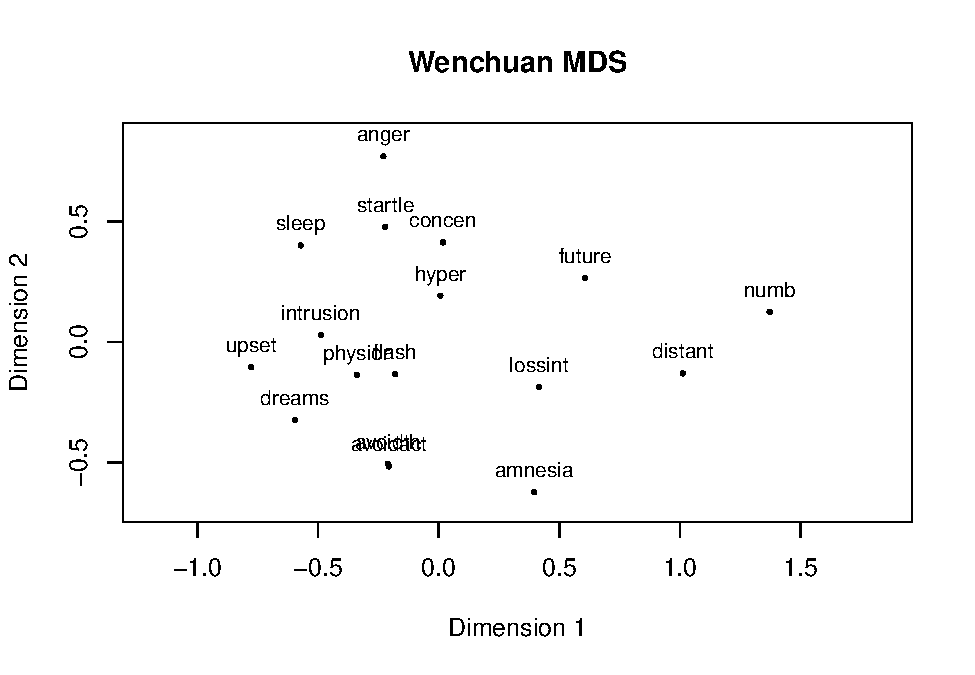
\includegraphics{LDA_files/figure-beamer/unnamed-chunk-29-1.pdf}

\hypertarget{right}{}
\begin{Shaded}
\begin{Highlighting}[]
\NormalTok{royston_test <-}\StringTok{ }\KeywordTok{mvn}\NormalTok{(}\DataTypeTok{data =}\NormalTok{ diabetes[,}\OperatorTok{-}\DecValTok{4}\NormalTok{], }\DataTypeTok{mvnTest =} \StringTok{"royston"}\NormalTok{, }\DataTypeTok{multivariatePlot =} \StringTok{"qq"}\NormalTok{)}
\end{Highlighting}
\end{Shaded}

Se pueden apreciar que existen outliers que prodían influenciar en el
contraste de normalidad multivariante.

\end{frame}

\begin{frame}[fragile]{Normalidad multivariante}

\hypertarget{left}{}
\begin{verbatim}
##      Test       H      p value MVN
## 1 Royston 113.878 2.120468e-25  NO
\end{verbatim}

\begin{verbatim}
##            Test       HZ p value MVN
## 1 Henze-Zirkler 9.215609       0  NO
\end{verbatim}

\hypertarget{right}{}
\begin{Shaded}
\begin{Highlighting}[]
\NormalTok{royston_test}\OperatorTok{$}\NormalTok{multivariateNormality}
\NormalTok{hz_test <-}\StringTok{ }\KeywordTok{mvn}\NormalTok{(}\DataTypeTok{data =}\NormalTok{ diabetes[,}\OperatorTok{-}\DecValTok{4}\NormalTok{], }\DataTypeTok{mvnTest =} \StringTok{"hz"}\NormalTok{)}
\NormalTok{hz_test}\OperatorTok{$}\NormalTok{multivariateNormality}
\end{Highlighting}
\end{Shaded}

\(H_0:\) El conjunto de datos sigue una distribución normal
multivariante

\(H_1:\) El conjunto de datos no sigue una distribución normal
multivariante

Ambos test muestran evidencias significativas de falta de normalidad
multivariante. El LDA tiene cierta robustez frente a la falta de
normalidad multivariante, pero es importante tenerlo en cuenta en la
conclusión del análisis.

\end{frame}

\begin{frame}[fragile]{Homogeneidad de Varianza}

\hypertarget{left}{}
\begin{verbatim}
## 
##  Box's M-test for Homogeneity of Covariance Matrices
## 
## data:  diabetes[, -4]
## Chi-Sq (approx.) = 290.13, df = 12, p-value < 2.2e-16
\end{verbatim}

\hypertarget{right}{}
\begin{Shaded}
\begin{Highlighting}[]
\KeywordTok{library}\NormalTok{(biotools)}
\KeywordTok{boxM}\NormalTok{(}\DataTypeTok{data =}\NormalTok{ diabetes[,}\OperatorTok{-}\DecValTok{4}\NormalTok{], }\DataTypeTok{grouping =}\NormalTok{ diabetes[,}\DecValTok{4}\NormalTok{])}
\end{Highlighting}
\end{Shaded}

\(H_0:\) La matriz de covarianza es igual en todos los grupos \(H_1:\)
La matriz de covarianza no es igual en todos los grupos El test Box's M
muestra evidencias de que la matriz de covarianza no es constante en
todos los grupos, lo que a priori descartaría el método LDA en favor del
QDA. Sin embargo, como el test Box's M es muy sensible a la falta de
normalidad multivariante, con frecuencia resulta significativo no porque
la matriz de covarianza no sea constante sino por la falta de
normalidad. Por esta razón se va a asumir que la matriz de covarianza sí
es constante y que LDA puede alcanzar una buena precisión en la
clasificación.

\end{frame}

\begin{frame}[fragile]{Análisis discriminante lineal2}

\hypertarget{left}{}
\begin{verbatim}
## Call:
## lda(class ~ ., data = diabetes)
## 
## Prior probabilities of groups:
## chemical   normal    overt 
## 0.226087 0.573913 0.200000 
## 
## Group means:
##            glucose   insulin     sspg
## chemical  99.46154  504.1154 291.7692
## normal    91.98485  351.2121 169.0152
## overt    207.17391 1002.9565 112.6087
## 
## Coefficients of linear discriminants:
##                  LD1          LD2
## glucose -0.035130542 -0.056150421
## insulin  0.013748266  0.009876402
## sspg     0.001344232  0.005489825
## 
## Proportion of trace:
##    LD1    LD2 
## 0.8526 0.1474
\end{verbatim}

\hypertarget{right}{}
\begin{Shaded}
\begin{Highlighting}[]
\KeywordTok{library}\NormalTok{(MASS)}
\NormalTok{modelo_lda2 <-}\StringTok{ }\KeywordTok{lda}\NormalTok{(class}\OperatorTok{~}\NormalTok{.,}\DataTypeTok{data=}\NormalTok{diabetes)}
\NormalTok{modelo_lda2}
\end{Highlighting}
\end{Shaded}

La función \texttt{lda} del paquete \texttt{MASS}. lda realiza la
clasificación mediante la aproximación de Fisher.

\end{frame}

\begin{frame}[fragile]{Evaluación de los errores de clasificación}

\hypertarget{left}{}
\begin{verbatim}
##           Clase predicha
## Clase real chemical normal overt
##   chemical       19      7     0
##   normal          1     65     0
##   overt           5      2    16
\end{verbatim}

\begin{verbatim}
## [1] "trainig_error = 13.0434782608696 %"
\end{verbatim}

De total de las observaciones 15 de las 115 predicciones que ha
realizado el modelo han sido erróneas. El trainig error es de (13.04\%).
Sin embargo, para validarlo es necesario un nuevo set de datos con el
que calcular el test error o recurrir a validación cruzada.

\hypertarget{right}{}
\begin{Shaded}
\begin{Highlighting}[]
\NormalTok{predicciones <-}\StringTok{ }\KeywordTok{predict}\NormalTok{(}\DataTypeTok{object =}\NormalTok{ modelo_lda2, }\DataTypeTok{newdata =}\NormalTok{ diabetes[}\OperatorTok{-}\DecValTok{4}\NormalTok{])}
\KeywordTok{table}\NormalTok{(diabetes}\OperatorTok{$}\NormalTok{class, predicciones}\OperatorTok{$}\NormalTok{class, }\DataTypeTok{dnn =} \KeywordTok{c}\NormalTok{(}\StringTok{"Clase real"}\NormalTok{, }\StringTok{"Clase predicha"}\NormalTok{))}

\NormalTok{trainig_error <-}\StringTok{ }\KeywordTok{mean}\NormalTok{(diabetes}\OperatorTok{$}\NormalTok{class }\OperatorTok{!=}\StringTok{ }\NormalTok{predicciones}\OperatorTok{$}\NormalTok{class) }\OperatorTok{*}\StringTok{ }\DecValTok{100}
\KeywordTok{paste}\NormalTok{(}\StringTok{"trainig_error ="}\NormalTok{, trainig_error, }\StringTok{"%"}\NormalTok{)}
\end{Highlighting}
\end{Shaded}

\end{frame}

\begin{frame}[fragile]{Visualización de las clasificaciones}

\begin{Shaded}
\begin{Highlighting}[]
\KeywordTok{library}\NormalTok{(klaR)}
\KeywordTok{partimat}\NormalTok{(class}\OperatorTok{~}\NormalTok{.,}\DataTypeTok{data=}\NormalTok{diabetes, }\DataTypeTok{method =} \StringTok{"lda"}\NormalTok{, }\DataTypeTok{prec =} \DecValTok{200}\NormalTok{,}
         \DataTypeTok{image.colors =} \KeywordTok{c}\NormalTok{(}\StringTok{"darkgoldenrod1"}\NormalTok{, }\StringTok{"snow2"}\NormalTok{, }\StringTok{"skyblue2"}\NormalTok{),}
         \DataTypeTok{col.mean =} \StringTok{"firebrick"}\NormalTok{,}\DataTypeTok{nplots.hor=}\DecValTok{3}\NormalTok{)       }
\end{Highlighting}
\end{Shaded}

La función \texttt{partimat()} del paquete \texttt{klar} permite
representar los límites de clasificación de un modelo discriminante
lineal o cuadrático para cada par de predictores. Cada color representa
una región de clasificación acorde al modelo, se muestra el centroide de
cada región y el valor real de las observaciones.

\end{frame}

\begin{frame}{Visualización de las clasificaciones}

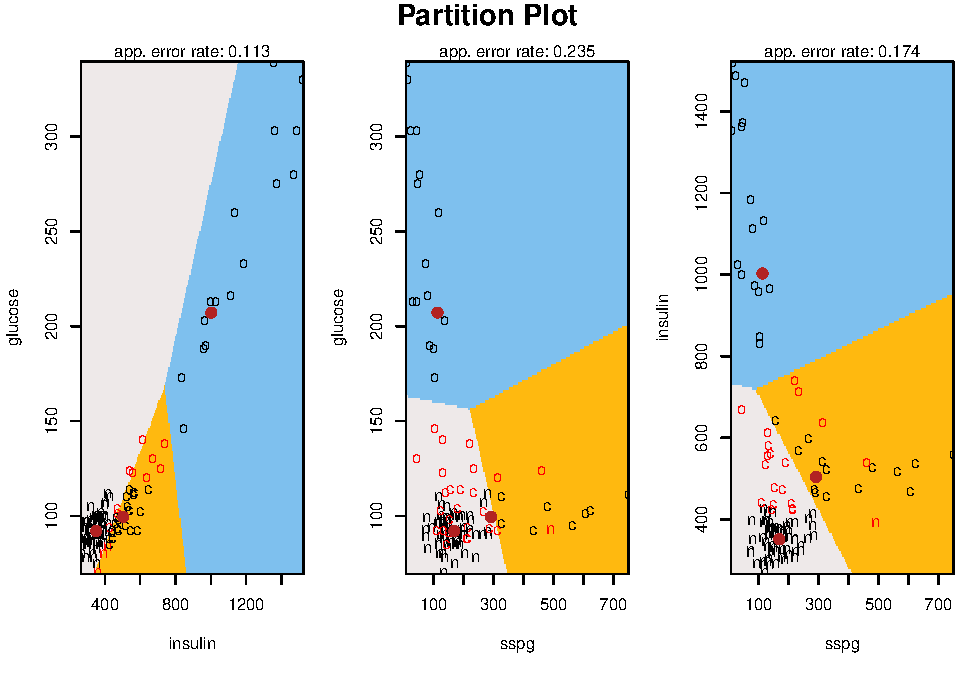
\includegraphics{LDA_files/figure-beamer/unnamed-chunk-34-1.pdf}

\end{frame}

\begin{frame}{Ejemplo 3}

El conjunto de datos, que contiene atributos y resultados en 1000
solicitudes de préstamo, fue proporcionado en 1994 por el Dr.~Hans
Hofmann, del Institut fuer Statistik und Oekonometrie de la Universidad
de Hamburgo. Ha servido como un importante conjunto de datos de prueba
para varios algoritmos de calificación crediticia. Las categorias de
clasificación son Default(Moroso): 0 (no) and 1 (si)

\end{frame}

\begin{frame}[fragile]{Cargando el conjunto de datos}

\begin{Shaded}
\begin{Highlighting}[]
\NormalTok{credit <-}\StringTok{ }\KeywordTok{read.csv}\NormalTok{(}\StringTok{"germancredit.csv"}\NormalTok{)}
\KeywordTok{head}\NormalTok{(credit,}\DecValTok{2}\NormalTok{)}
\end{Highlighting}
\end{Shaded}

\begin{verbatim}
##   Default checkingstatus1 duration history purpose amount savings employ
## 1       0             A11        6     A34     A43   1169     A65    A75
## 2       1             A12       48     A32     A43   5951     A61    A73
##   installment status others residence property age otherplans housing
## 1           4    A93   A101         4     A121  67       A143    A152
## 2           2    A92   A101         2     A121  22       A143    A152
##   cards  job liable tele foreign
## 1     2 A173      1 A192    A201
## 2     1 A173      1 A191    A201
\end{verbatim}

Como se puede ver, solo las variables: duración (\texttt{duration}),
monto (\texttt{amount}), plazo (\texttt{installment}) y edad
(\texttt{age}) son numéricas. Con los restantes (indicadores), las
suposiciones de una distribución normal serían, en el mejor de los
casos, débiles; por lo tanto estas variables no son consideradas aquí.

\end{frame}

\begin{frame}[fragile]{Conjunto de datos final}

\begin{Shaded}
\begin{Highlighting}[]
\NormalTok{cred1=credit[, }\KeywordTok{c}\NormalTok{(}\StringTok{"Default"}\NormalTok{,}\StringTok{"duration"}\NormalTok{,}\StringTok{"amount"}\NormalTok{,}\StringTok{"installment"}\NormalTok{,}\StringTok{"age"}\NormalTok{)]}
\KeywordTok{head}\NormalTok{(cred1)}
\end{Highlighting}
\end{Shaded}

\begin{verbatim}
##   Default duration amount installment age
## 1       0        6   1169           4  67
## 2       1       48   5951           2  22
## 3       0       12   2096           2  49
## 4       0       42   7882           2  45
## 5       1       24   4870           3  53
## 6       0       36   9055           2  35
\end{verbatim}

\end{frame}

\begin{frame}[fragile]{Normalidad multivariante}

\hypertarget{left}{}
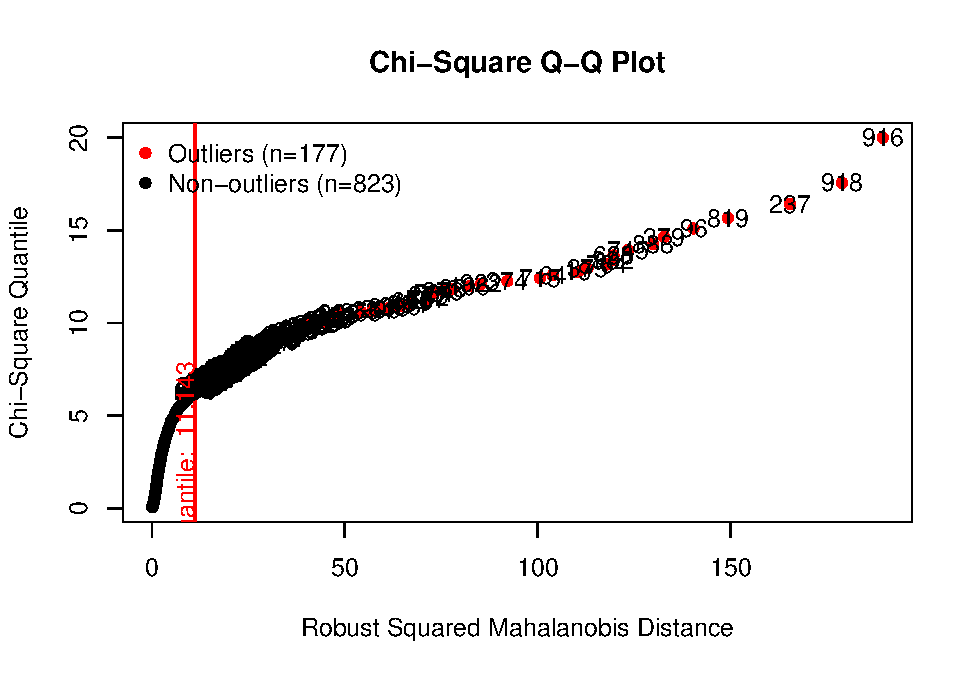
\includegraphics{LDA_files/figure-beamer/unnamed-chunk-37-1.pdf}

\hypertarget{right}{}
\begin{Shaded}
\begin{Highlighting}[]
\KeywordTok{library}\NormalTok{(MVN)}
\NormalTok{outliers <-}\StringTok{ }\KeywordTok{mvn}\NormalTok{(}\DataTypeTok{data =}\NormalTok{ cred1[,}\OperatorTok{-}\DecValTok{1}\NormalTok{], }\DataTypeTok{mvnTest =} \StringTok{"hz"}\NormalTok{, }\DataTypeTok{multivariateOutlierMethod =} \StringTok{"quan"}\NormalTok{)}
\end{Highlighting}
\end{Shaded}

Existen \(n=117\) outliers que prodían influenciar en el contraste de
normalidad multivariante.

\end{frame}

\begin{frame}[fragile]{Normalidad multivariante}

\hypertarget{left}{}
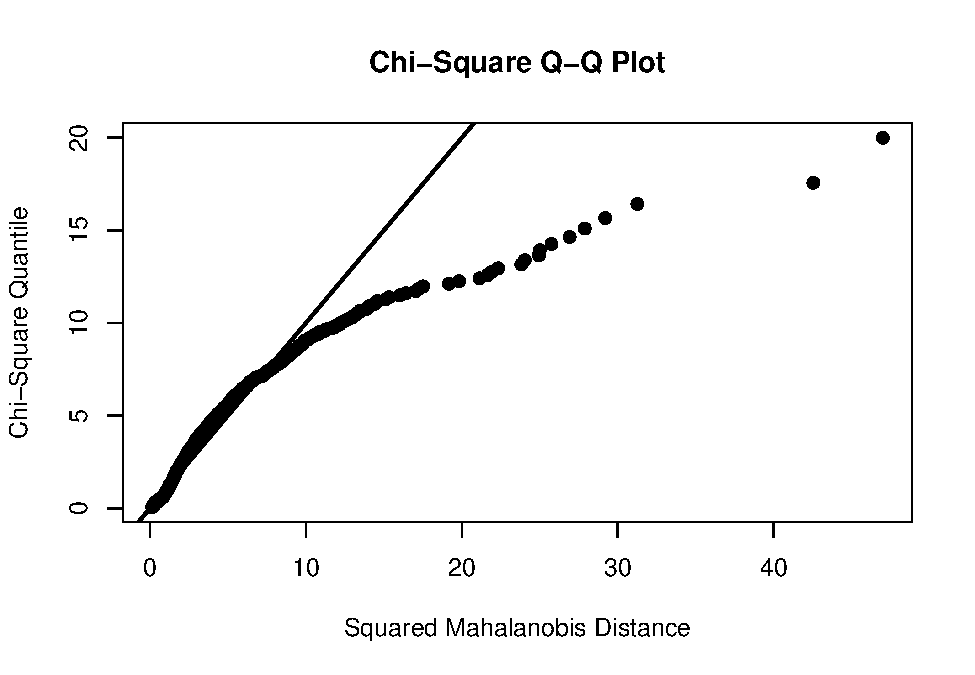
\includegraphics{LDA_files/figure-beamer/unnamed-chunk-38-1.pdf}

\hypertarget{right}{}
\begin{Shaded}
\begin{Highlighting}[]
\NormalTok{royston_test <-}\StringTok{ }\KeywordTok{mvn}\NormalTok{(}\DataTypeTok{data =}\NormalTok{ cred1[,}\OperatorTok{-}\DecValTok{1}\NormalTok{], }\DataTypeTok{mvnTest =} \StringTok{"royston"}\NormalTok{, }\DataTypeTok{multivariatePlot =} \StringTok{"qq"}\NormalTok{)}
\end{Highlighting}
\end{Shaded}

Se pueden apreciar que existen outliers que prodían influenciar en el
contraste de normalidad multivariante.

\end{frame}

\begin{frame}[fragile]{Normalidad multivariante}

\hypertarget{left}{}
\begin{verbatim}
##      Test       H       p value MVN
## 1 Royston 498.872 1.184884e-106  NO
\end{verbatim}

\begin{verbatim}
##            Test       HZ p value MVN
## 1 Henze-Zirkler 17.40368       0  NO
\end{verbatim}

\hypertarget{right}{}
\begin{Shaded}
\begin{Highlighting}[]
\NormalTok{royston_test}\OperatorTok{$}\NormalTok{multivariateNormality}
\NormalTok{hz_test <-}\StringTok{ }\KeywordTok{mvn}\NormalTok{(}\DataTypeTok{data =}\NormalTok{ cred1[,}\OperatorTok{-}\DecValTok{1}\NormalTok{], }\DataTypeTok{mvnTest =} \StringTok{"hz"}\NormalTok{)}
\NormalTok{hz_test}\OperatorTok{$}\NormalTok{multivariateNormality}
\end{Highlighting}
\end{Shaded}

\(H_0:\) El conjunto de datos sigue una distribución normal
multivariante

\(H_1:\) El conjunto de datos no sigue una distribución normal
multivariante

Los datos no siguen una distribución normal multivariante, lo que tiene
implicaciones directas en la precisión del QDA.

\end{frame}

\begin{frame}[fragile]{Homogeneidad de Varianza}

\hypertarget{left}{}
\begin{verbatim}
## 
##  Box's M-test for Homogeneity of Covariance Matrices
## 
## data:  cred1[, -1]
## Chi-Sq (approx.) = 160.06, df = 10, p-value < 2.2e-16
\end{verbatim}

\hypertarget{right}{}
\begin{Shaded}
\begin{Highlighting}[]
\KeywordTok{library}\NormalTok{(biotools)}
\KeywordTok{boxM}\NormalTok{(}\DataTypeTok{data =}\NormalTok{ cred1[,}\OperatorTok{-}\DecValTok{1}\NormalTok{], }\DataTypeTok{grouping =}\NormalTok{ cred1[,}\DecValTok{1}\NormalTok{])}
\end{Highlighting}
\end{Shaded}

\(H_0:\) La matriz de covarianza es igual en todos los grupos \(H_1:\)
La matriz de covarianza no es igual en todos los grupos El test Box's M
muestra mucha evidencia de que la matriz de covarianza no es constante
en todos los grupos, esta condición hace que el QDA sea más adecuado.

\end{frame}

\begin{frame}[fragile]{Anáslisis de discriminante cuadrático}

\hypertarget{left}{}
\begin{Shaded}
\begin{Highlighting}[]
\KeywordTok{library}\NormalTok{(MASS)}
\NormalTok{modelo_qda <-}\StringTok{ }\KeywordTok{qda}\NormalTok{(}\DataTypeTok{formula =}\NormalTok{ Default}\OperatorTok{~}\NormalTok{., }\DataTypeTok{data =}\NormalTok{ cred1)}
\NormalTok{modelo_qda}
\end{Highlighting}
\end{Shaded}

\hypertarget{right}{}
\begin{verbatim}
## Call:
## qda(Default ~ ., data = cred1)
## 
## Prior probabilities of groups:
##   0   1 
## 0.7 0.3 
## 
## Group means:
##   duration   amount installment      age
## 0 19.20714 2985.457    2.920000 36.22429
## 1 24.86000 3938.127    3.096667 33.96333
\end{verbatim}

\end{frame}

\begin{frame}[fragile]{Clasificación de nuevas observaciones}

\begin{Shaded}
\begin{Highlighting}[]
\NormalTok{zqua=}\KeywordTok{qda}\NormalTok{(Default}\OperatorTok{~}\NormalTok{.,cred1)}
\KeywordTok{predict}\NormalTok{(zqua,}\DataTypeTok{newdata=}\KeywordTok{data.frame}\NormalTok{(}\DataTypeTok{duration=}\DecValTok{6}\NormalTok{,}\DataTypeTok{amount=}\DecValTok{1100}\NormalTok{,}\DataTypeTok{installment=}\DecValTok{4}\NormalTok{,}\DataTypeTok{age=}\DecValTok{67}\NormalTok{))}
\end{Highlighting}
\end{Shaded}

\begin{verbatim}
## $class
## [1] 0
## Levels: 0 1
## 
## $posterior
##           0          1
## 1 0.9375556 0.06244441
\end{verbatim}

La probabilidad posterior de que el cliente sea moroso del 6.24\% frente
al 93.76\% de que no sea moroso.

\end{frame}

\begin{frame}[fragile]{Evaluación de los errores de clasificación}

\hypertarget{left}{}
\begin{verbatim}
##           Clase predicha
## Clase real   0   1
##          0 628  72
##          1 221  79
\end{verbatim}

\begin{verbatim}
## [1] "trainig_error = 29.3 %"
\end{verbatim}

De total de las observaciones 293 de las 1000 predicciones que ha
realizado el modelo han sido erróneas. El trainig error es de (29.3\%).
Sin embargo, para validarlo es necesario un nuevo set de datos con el
que calcular el test error o recurrir a validación cruzada.

\hypertarget{right}{}
\begin{Shaded}
\begin{Highlighting}[]
\NormalTok{predicciones <-}\StringTok{ }\KeywordTok{predict}\NormalTok{(}\DataTypeTok{object =}\NormalTok{ modelo_qda, }\DataTypeTok{newdata =}\NormalTok{ cred1)}
\KeywordTok{table}\NormalTok{(cred1}\OperatorTok{$}\NormalTok{Default, predicciones}\OperatorTok{$}\NormalTok{class,}
      \DataTypeTok{dnn =} \KeywordTok{c}\NormalTok{(}\StringTok{"Clase real"}\NormalTok{, }\StringTok{"Clase predicha"}\NormalTok{))}

\NormalTok{trainig_error <-}\StringTok{ }\KeywordTok{mean}\NormalTok{(cred1}\OperatorTok{$}\NormalTok{Default }\OperatorTok{!=}\StringTok{ }\NormalTok{predicciones}\OperatorTok{$}\NormalTok{class) }\OperatorTok{*}\StringTok{ }\DecValTok{100}
\KeywordTok{paste}\NormalTok{(}\StringTok{"trainig_error ="}\NormalTok{, trainig_error, }\StringTok{"%"}\NormalTok{)}
\end{Highlighting}
\end{Shaded}

\end{frame}

\begin{frame}{Referencias}

\begin{itemize}
\item
  \url{http://halweb.uc3m.es/esp/Personal/personas/jmmarin/esp/DM/tema1dm.pdf}
\item
  \url{https://rstudio-pubs-static.s3.amazonaws.com/35817_2552e05f1d4e4db8ba87b334101a43da.html}
\item
  \url{https://rpubs.com/Joaquin_AR/233932}
\end{itemize}

\end{frame}

\end{document}
